\documentclass[10pt,journal,compsoc]{IEEEtran}
\usepackage{cite}
\usepackage{graphicx}
\usepackage{psfrag}

\usepackage{url}
\usepackage{color}
\usepackage{balance}
\usepackage[all]{xy}
\usepackage{xspace}
\usepackage{listings}
\usepackage{adjustbox}
\usepackage{array,booktabs,arydshln,xcolor}
\usepackage{tikz}

\usetikzlibrary{shapes,patterns,calc,shapes.geometric,arrows}
\usepackage{makecell}
\usepackage{multirow}
\usepackage{xcolor}
\usepackage{url}
\usepackage{amsthm}
% \usepackage{pgfplots}
\usepackage{float}
\usepackage{amsmath}
\usepackage[capitalise]{cleveref}
\usepackage{soul}
\usepackage[inline]{enumitem}
\usepackage{xcolor}
\usepackage{amssymb}
\usepackage{pifont}

\usepackage{subcaption}
\graphicspath{{Images/}}
\definecolor{commentsColor}{rgb}{0.497495, 0.497587, 0.497464}
\definecolor{keywordsColor}{rgb}{0.000000, 0.000000, 0.635294}
\definecolor{stringColor}{rgb}{0.558215, 0.000000, 0.135316}
\theoremstyle{definition}
\newtheorem{definition}{Definition}[section]
\newtheorem{theorem}{Theorem}[section]
%\newtheorem{problem}{Problem}[section]
\newtheorem{example}{Example}[section]
\newcommand{\xmark}{\ding{55}}%
\newcommand{\cmark}{\ding{51}}%
\newcommand{\chia}[1]{{\color{red}#1}}
% please place your own definitions here and don't use \def but
% \newcommand{}{}
\newcommand\CH[1]{\textcolor{blue}{{CHIARA - }{#1}}}
\newcommand\CL[1]{\textcolor{red}{{CLAUDIO - }{#1}}}
\newcommand\MC[1]{\textcolor{green}{{MARCO - }{#1}}}
\newcommand\AG[1]{\textcolor{orange}{{AG - }{#1}}}
\newcommand{\job}[1]{\ensuremath{J_{#1}}}
\newcommand{\trans}[1]{\ensuremath{T_{#1}}}
\newcommand{\coalition}[1]{\ensuremath{C_{#1}}}
\newcommand{\org}[1]{\ensuremath{o_{#1}}}
\newcommand{\Org}[1]{\ensuremath{O_{#1}}}
\newcommand{\s[1]}{\ensuremath{s_{}}}
\newcommand{\si}[1]{\ensuremath{s_{#1}}}
\newcommand{\sii}[1]{\ensuremath{s'_{#1}}}
\newcommand{\dataset}[1]{\ensuremath{D_{#1}}}
\newcommand{\origdataset}{\ensuremath{X}}
\newcommand{\transdataset}{\ensuremath{Y}}

\newcommand{\T}{\ensuremath{T}}
\newcommand{\TP}{\ensuremath{T^{P}}}
\newcommand{\TF}[1]{\ensuremath{T^F_{#1}}}
\newcommand{\tf}[1]{\ensuremath{t^f_{#1}}}
\newcommand{\tp}[1]{\ensuremath{t^p_{#1}}}

\newcommand{\G}{\ensuremath{G}}

\newcommand{\F}[1]{\ensuremath{F_{#1}}}

\newcommand{\plusOperator}{\ensuremath{\oplus}}
\newcommand{\timesOperator}{\ensuremath{\otimes}}

\newcommand{\V}{\ensuremath{V}}
\newcommand{\Vp}{\ensuremath{V'}}
\newcommand{\Vplus}{\ensuremath{V_{\plusOperator}}}
\newcommand{\Vtimes}{\ensuremath{V_{\timesOperator}}}
\newcommand{\Vpplus}{\ensuremath{V'_{\plusOperator}}}
\newcommand{\Vptimes}{\ensuremath{V'_{\timesOperator}}}

\newcommand{\vi}[1]{\ensuremath{v_{#1}}}
\newcommand{\vii}[1]{\ensuremath{v'_{#1}}}

\newcommand{\E}{\ensuremath{E}}

\newcommand{\myLambda}{\ensuremath{\lambda}\,}
\newcommand{\myGamma}{\ensuremath{\gamma}\,}
\newcommand{\templateChartAnnotation}{\ensuremath{\myLambda,\myGamma}}
\newcommand{\instanceChartAnnotation}{\ensuremath{\myLambda}}
\renewcommand{\P}[1]{\ensuremath{P_{#1}}}
\newcommand{\p}[1]{\ensuremath{p_{#1}}}
% \newcommand{\TF}{\ensuremath{T_{\fChartFunction}}}
\newcommand{\user}{user\,}
\newcommand{\User}{User\,}
\newcommand{\profile}{\emph{prf}}

\newcommand{\fChartFunction}{\ensuremath{\myLambda{}}}

\newcommand{\tChartFunction}{\ensuremath{G^{\myLambda,\myGamma}(\V,\E,\myLambda,\myGamma)}\xspace}
% \newcommand{\iChartFunction}{\ensuremath{\fChartFunction,\myGamma{},\myLambda{}}}
\newcommand{\iChartFunction}{\ensuremath{G'(\V',\E,\myLambda)}\xspace}



\newcommand{\pipeline}{Pipeline\xspace}
\newcommand{\pipelineTemplate}{Pipeline Template\xspace}
\newcommand{\pipelineInstance}{Pipeline Instance\xspace}



\newcommand{\problem}{Pipeline Instantiation Process }

\newcommand{\policy}[5]{
  $\langle \text{#1},{#2},{#3},\ensuremath{#4},\ensuremath{#5} \rangle$
}

\begin{document}

\title{TBA}

\author{Marco Anisetti~\IEEEmembership{Senior Member,~IEEE,}, Claudio A. Ardagna~\IEEEmembership{Senior Member,~IEEE,} Chiara Braghin, Ernesto Damiani~\IEEEmembership{Senior Member,~IEEE,}, Antongiacomo Polimeno % <-this % stops a space
  \IEEEcompsocitemizethanks{\IEEEcompsocthanksitem M. Anisetti, C.A. Ardagna, E. Damiani, are with the Dipartimento di Informatica, Universit\`a degli Studi di Milano, Milano,
    Italy. E. Damiani is also with.\protect\\
    E-mail: \{firstname.lastname\}@unimi.it
  }
  \thanks{}}

%\markboth{~}{~}

\IEEEcompsoctitleabstractindextext{%
  \begin{abstract}
    The conflict between the need of protecting and sharing data is hampering the spread of big data applications. Proper security and privacy assurance is required to protect data owners, while proper data access and sharing are fundamental to implement smart big data solutions. In this context, access control systems assume a central role for balancing the need of data protection and sharing. However, given the software and technological complexity of big data ecosystems, existing solutions are not suitable because they are neither general nor scalable, and do not support a dynamic and collaborative environment. In this paper, we propose an access control system that enforces access to data in a distributed, multi-party big data environment. It is based on data annotations and secure data transformations performed at ingestion time. We show the feasibility of our approach with a case study in a smart city domain using an Apache-based big data engine.

  \end{abstract}

  \begin{IEEEkeywords}
    Access Control, Big Data, Data Transformation, Data Ingestion
  \end{IEEEkeywords}}

\maketitle

\IEEEdisplaynotcompsoctitleabstractindextext

\IEEEpeerreviewmaketitle

\tikzset{
  do path picture/.style={%
      path picture={%
          \pgfpointdiff{\pgfpointanchor{path picture bounding box}{south west}}%
          {\pgfpointanchor{path picture bounding box}{north east}}%
          \pgfgetlastxy\x\y%
          \tikzset{x=\x/2,y=\y/2}%
          #1
        }
    },
  cross/.style={do path picture={
          \draw [line cap=round ] (-1,-1) -- (1,1) (-1,1) -- (1,-1);
        }},
  plus/.style={do path picture={
          \draw [line cap=round] (-3/4,0) -- (3/4,0) (0,-3/4) -- (0,3/4);
        }}
}

\section{Introduction}
TBW
\section{Motivations}
Data quality is a largely studied research topic. The database management research community mainly focused on increasing the quality of the source data rather than guaranteeing data quality along the whole processing pipeline or the quality of outcomes built on data.
In \cite{BigDataQaulitySurvey} a survey on big data quality is proposed mentioning the well known categories of big data quality grouped by intrinsic,
contextual representational and accessibility categories.
It also presents an holistic quality management model where the importance of data quality during processing is just mentioned in terms of requirements for the pre-processing job (e.g., data enhancement due to cleaning jobs).
In this paper we depart from this idea on data quality at pre processing time only measuring it at each step of the big data pipeline.
%data quality are divided into four categories: intrinsic, contextual representational and accessibility that covers almost all the aspects of data at ingestion time

\subsection{Background}
\subsection{Data Protection}
Research on data governance and protection focuses on the definition of new approaches and techniques aimed to protect the security and privacy of big data (e.g., CIA triad), as well as managing their life cycle with security and privacy in mind. Often, the research community is targeting specific security and privacy problems, resulting in a proliferation of solutions and tools, which are difficult to integrate in a coherent framework. Many solutions have been developed to protect the users' identity (e.g., anonymity \cite{wallace1999anonymity}, pseudonimity \cite{pfitzmann2001pseudonymity}, k-anonymity \cite{k-anon}), to guarantee data confidentiality and integrity (e.g., encryption \cite{thambiraja2012survey}, differential privacy \cite{hassan2019differential}, access control \cite{tolone2005access,servos2017current}), and to govern data sharing and analysis (e.g., data lineage \cite{woodruff1997supporting}, ETL/ELT ingestion \cite{vassiliadis2009survey}).

This project proposal focuses on access control, an approach adopted to protect access to data from unauthorized users from the very beginning of ICT systems. Coming to big data, most of the current solution leverage on Attribute-Based Access Control (ABAC) \cite{NIST:ABAC:2014} to manage policy rules adaptable at run time using attributes. In general, these systems must be instantiated on the specific scenario of interest and are ineffective when complexity increase due to the computational overhead and introduction of delays in policy enforcement. There are also database-centric approaches that focus on specific databases such as noSQL databases or graph databases, or specific types of analytical pipelines such \cite{AConGraphDB:2021, AConMongoDB:2022, ABACforHBase:2019}. However, these solutions are widely based on query rewriting mechanisms leading to high complexity and low efficiency. Finally, some solutions are scenario-specific (federate cloud, edge microservices or IoT) and lack the generality needed to adapt to multiple contexts \cite{MultipartyAC:2019, IoTSecurity}.
The closest approach to this project proposal is the work of Hu et al. \cite{ HUFerraiolo:2014}, introducing a generalized access control model for big data processing frameworks, which can be extended to the Hadoop environment. However, the paper discusses the issues only from a high-level architectural point of view, without discussing a tangible solution. Another relevant work is by Xue et al. \cite{GuardSpark:ACSAC:2020}. They propose a solution based on the notion of purpose-aware access control \cite{Byun2008} that, although focusing only on Apache Spark, recognizes the need of a generalized approach to deal with access control in analytics pipelines.

An effective data governance and protection approach cannot avoid its integration within state-of-the-art big data infrastructures. In fact, as organizations see practical results and significant value in the usage of big data, they also recognize the limits of current big data ecosystems with respect to data governance and data protection. Recently, both industry and academic communities started to investigate the issue, both from a data governance perspective \cite{al2018exploring,aissa2020decide} or recognizing the need of new security requirements \cite{Colombo:JournCybersec:2019}. Although Attribute Based Access Control (ABAC) \cite{NIST:ABAC:2014} is currently adopted in big data projects as a common underlying model given its ability to support highly flexible and dynamic forms of data protection to business-critical data, the dynamic and decentralized nature of big data asks for new solutions. Actual solutions are neither general nor scalable, since they are either platform-dependent or coarse-grained \cite{Colombo:JournCybersec:2019}.
%
Platform-specific approaches are designed for single systems only (e.g., MongoDB, Hadoop) and leverage on native access control features of the platform \cite{rathore2017hadoop,anisetti2018privacy}.
Some recent proposals, like Federated Access Control Reference Model (FACRM) \cite{FederationAC:Journ:2020} or \cite{Sandhu:ABAC:2018,GuptaSandu:2017}, are specifically tailored to the Apache Hadoop stack.
On the other hand, platform-independent approaches have the advantage of being more general than platform-specific solutions. However, the currently available platforms either model resources to be accessed as monolithic files (e.g., Microsoft DAC) or lack scalability.

Finally, the success of big data and the increasing central role of data in our everyday life increased the attention also by institutions and public administrations resulting in new regulations and guidelines.
%
The possibility of using data indiscriminately by analyzing and sharing them has led to the emergence of specific and stringent regulations such as the General Data Protection Regulation (GDPR)\cite{gdpr}. GDPR is the first and best known of a series of regulations that aim to achieve this goal. GDPR enforced in 2018, replaced the inadequate Data Protection Directive 95/46/EC. GDPR was intended to raise awareness of companies and consumers on security, privacy and the right to be forgotten.
%
The enormous growth of machine learning technologies and their pervasive diffusion, has led to the idea that artificial intelligence was also a field to be regulated. On 8 April 2019, the High-Level Expert Group on AI presented Ethics Guidelines for Trustworthy Artificial Intelligence, which proposes the development of reliable AI, that is: lawful, robust and ethical \cite{euai}.
%
Finally, the problem of guaranteeing data sovereignty clearly emerged and is leading EU commission activities \cite{pedreira2021review}. In this context, project Gaia-X, presented in October 2019 by the German and French Ministries of Economic Affairs, gathered more than 5,000 participants in one year. The project aims to satisfy a widespread need of European countries to regain possession of the sovereignty of their data, facilitate the creation of interconnected data spaces that comply with compliance criteria, open-source software, providing certification tools \cite{gaiax}. Another example of work on the data sovereignty topic is the development of the European Data Governance Act that is currently underway and aims to regulate and encourage data sharing within the European Union \cite{edca}.
\subsection{Data Processing}
The need of analyzing and extracting value from data emerged from the very beginning of ICT,
and is at the basis of a vast research area that includes database technologies \cite{palanisamy2020survey},
data mining \cite{jain2013data,castano2017exploratory},
big data analytics \cite{tsai2015big} and machine learning \cite{qiu2016survey}.
This project proposal focuses on machine learning in the context of modern big data infrastructures.
Research on machine learning focused on many aspects of data learning and analysis,
and is horizontal to multiple domains and research areas.
Machine learning has evolved from simple mining based on logistic regression and naive Bayes to Deep Learning,
via Decision tree and linear regression.
Deep learning is a subset of Neural Network techniques,
which owe their success to the ever increasing computational power and massive amount of data available.
Deep Learning copes well with the distribution of computations reaching excellent performances thanks to the work done in the parallelization of machine learning processing \cite{verbraeken2020survey, Goodfellow-et-al-2016,wu2022survey}.

At the same time, substantial research and development effort has been put on the infrastructures supporting data analysis, which underwent a gradual evolution starting from a monolithic model towards a model based on micro and nano services \cite{kratzke2018brief}. The spread of the cloud computing and  containerized systems allowed these systems to be more resilient, easier to develop, and adaptive, while increasing their complexity.\footnote{Today the Apache big data ecosystem counts more than 50 tools.}
With the spread of big data, new tools and infrastructures have been developed for data ingestion, storage, and analysis. The main challenge to be addressed was the inability for a single system to handle such huge amount of data; this resulted in the spread of solutions based on a distributed file system \cite{blomer2015survey}, a system that permits to share data across multiple machines (made in general of commodity hardware), making possible for the user to read and write data without perceiving this distribution. Over the years these systems have seen more and more refinements and expansions, such as, resource managers to manage the distribution of resources in the network of nodes (YARN) \cite{kulkarni2014survey}, SQL-Like systems that support access following standard RDBMS (HIVE, Presto, Trino) \cite{thusoo2009hive,sethi2019presto}. Finally, other software components (for example Apache Spark \cite{salloum2016big}) have been created to meet the ever increasing needs for data access and analysis requested by machine learning technologies.

\section{System Model and Service Pipeline}\label{sec:requirements}
Big data is highly dependent on cloud-edge computing, which makes extensive use of multitenancy.
Multitenancy permits sharing one instance of infrastructures, platforms or applications by multiple tenants to optimize costs. This leads to common scenarios where a service provider offers subscription-based analytics capabilities in the cloud, or a single data lake is accessed by multiple customers. Big data pipelines then mix data and services which belong to various organizations, posing a serious risk of potential privacy and security violations.

We propose a data governance framework tailored to contemporary data-driven pipelines, which aims to limit the privacy and security risks. The primary objective of this framework is to facilitate the assembly of data processing services, with a central focus on the selection of those services that optimize data quality, while upholding privacy and security requirements.

In the following of this section, we present our system model (Section \ref{sec:systemmodel}) and our reference scenario (Section \ref{sec:service_definition}).

\subsection{System Model}\label{sec:systemmodel}
In today's data landscape, the coexistence of data quality and data privacy is critical to support high-value services and pipelines. The increase in data production, collection, and usage has led to a split in scientific research priorities.
%This has resulted in two main focus areas.
First, researchers are exploring methods to optimize the usage of valuable data. Here, ensuring data quality is vital, and requires accuracy, reliability, and soundness for analytical purposes.
Second, there is a need to prioritize data privacy and security. This involves safeguarding confidential information and complying with strict privacy regulations. These two research directions are happening at the same time, though there are not many solutions that find a good balance between them.

Our approach seeks to harmonize these objectives by establishing a data governance framework that balances privacy and data quality. It implements a system model that is composed of the following parties:
\begin{description}
  \item[Service,] a software distributed by a \textbf{service provider} that performs a specific task according to access control privileges on data; %, a service can be tagged with some policies %, a service is characterized by two function: the service function and the policy function.
  \item[Pipeline,] a sequence of connected services that collect, prepare, process, and analyze data in a structured and automated manner. We distinguish between a \textbf{pipeline template} that acts as a skeleton, specifying the structure of the pipeline and the (non-)functional requirements driving service selection and composition, and a \textbf{pipeline instance} instantiating the template with services according to the specified requirements;
  \item[Data Governance Policy,] a structured set of privacy guidelines, rules, and procedures regulating data access and protection;
  \item[User] that executes an analytics pipeline on the data. We assume that the data target of the analytics pipeline are ready for analysis, that is, they underwent a preparatory phase addressing issues such as missing values, outliers, and formatting discrepancies. This ensures that the data are in an optimal state for subsequent analysis.
\end{description}

%The \user starts its analytics by first selecting a pipeline template among a set of functionally-equivalent templates. The template is selected according to the \user\ non-functional requirements and then instantiated in a pipeline instance. In particular, for each component service in the template, a real service is selected among a list of compatible services in the instance. Compatible services are functionally equivalent and comply with the privacy policies specified in the template.
The \user first selects a pipeline template among a set of functionally-equivalent templates according to its non-functional requirements. It then instantiates the template in a pipeline instance. To this aim, for each component service in the template, it retrieves a set of candidate services that satisfy the functional requirements of the component service. Candidate services are filtered to retrieve a list of compatible services that comply with the  policies specified in the template.

Compatible services are ranked based on their ability to retain the maximum amount of information (\emph{data quality} in this paper), while maintaining a minimum level of privacy; the best service is then selected to instantiate the corresponding component service in the template.
Upon selecting the most suitable service for each component service in the pipeline template, the pipeline instance is completed and ready for execution.
It is important to note that our data governance approach builds on the following assumption: \emph{upholding a larger quantity of data is linked to better data quality.}
While this assumption is not true in all settings, it correctly represents many real-world scenarios. We leave a solution that departs from this assumption to our future work.

\subsection{Service Pipeline and Reference Scenario}\label{sec:service_definition}
We consider a service-based environment where a service pipeline is designed to analyze data.
We define a service pipeline as a graph defined as follows. % and depicted in \cref{fig:service_pipeline}.
\begin{definition}[\pipeline]\label{def:pipeline}
  % A \pipeline is as a direct acyclic graph G(\V,\E), where \V\ is a set of vertices and \E\ is a set of edges connecting two vertices \vi{i},\vi{k}$\in$\V. The graph has a root \vi{r}$\in$\V, a vertex \vi{i}$\in$\V$_S$ for each service $s_i$, two additional vertices \vi{c},\vi{m}$\in$\V$_{\timesOperator}$$\subset$\V\ for each alternative ($\timesOperator$) structure modeling the alternative execution (\emph{choice}) of operations and the retrieval (\emph{merge}) of the results, respectively, and one additional vertex \vi{f} $\in$\V$_{\plusOperator}$$\subset$\V\ for each parallel ($\plusOperator$) structure modeling the contemporary execution (\emph{fork}) of operations.
  A \pipeline is as a direct acyclic graph G(\V,\E), where \V\ is a set of vertices and \E\ is a set of edges connecting two vertices \vi{i},\vi{k}$\in$\V.
  The graph has a root \vi{r}$\in$\V, a vertex \vi{i}$\in$\V$_S$ for each service $s_i$, an additional vertex \vi{f}$\subset$\V\ for each parallel ($\plusOperator$) structure modeling the contemporary execution (\emph{fork}) of services.
\end{definition}

We note that \{\vi{r},\vi{f}\}$\cup$\V$_S$$=$\V, vertices \vi{f} model branching for parallel structures, and root \vi{r} possibly represents the orchestrator. We also note that, for simplicity but no lack of generality, alternative structures modeling the alternative execution of services are specified as alternative service pipelines, that is, there is no alternative structure in a single service pipeline.

% A service pipeline is as a direct acyclic graph G(\V,\E), where \V\ is a set of vertices, one for each service $s_i$ in the pipeline, \E\ is a set of edges connecting two services $s_i$ and $s_j$, and \myLambda\ is an annotation function that assigns a label \myLambda(\vi{i}), corresponding to a data transformation \F\ implemented by the service $s_i$, for each vertex \vi{i}$\in$\V.
Our reference scenario considers a service pipeline analyzing a dataset of individuals detained in Department of Correction facilities in the state of Connecticut while awaiting trial \cite{toadd}.
In particular, the user, a member of the Connecticut Department of Correction (DOC), seeks to compare admission trends in Connecticut prisons with DOCs in New York and New Hampshire. We assume DOCs to be partners and share data according to their privacy policies.
The user's preferences align with a predefined pipeline template that orchestrates the following sequence of operations:
\begin{enumerate*}[label=(\roman*)]
  \item \emph{Data fetching}, including the download of the dataset from other states;
  \item \emph{Data preparation}, including data merging, cleaning, and anonymization;
        % \hl{QUESTO E' MERGE (M). IO PENSAVO DIVENTASSE UN NODO $v_i$. NEL CASO CAMBIANDO LA DEFINIZIONE 3.1 DOVE NON ESISTONO PIU' I NODI MERGE E JOIN.}
  \item \emph{Data analysis}, including statistical measures like average, median, and clustering-based statistics;
  \item \emph{Data storage}, including the storage of the results;
  \item \emph{Data visualization}, including the visualization of the results.
\end{enumerate*}

We note that the template requires the execution of the entire service within the Connecticut Department of Correction. If the data needs to be transmitted beyond the boundaries of Connecticut, data protection measures must be implemented. A visual representation of the flow is presented in Figure \ref{fig:reference_scenario}.
%
\cref{tab:dataset} presents a sample of the adopted dataset.\footnote{https://data.ct.gov/Public-Safety/Accused-Pre-Trial-Inmates-in-Correctional-Faciliti/b674-jy6w} Each row represents an inmate; each column includes the following attributes: date of download, a unique identifier, last entry date, race, gender, age of the individual, the bound value, offense, entry facility, and detainer. To serve the objectives of our study, we have extended this dataset by introducing randomly generated first and last names.

\begin{table*}[ht!]
  \caption{Dataset sample}
  \label{tab:dataset}
  \centering
  \begin{adjustbox}{max totalsize={.99\linewidth}{\textheight},center}
    \bgroup
    \def\arraystretch{1.5}
    \begin{tabular}{|l|l|l|l|l|l|l|l|l|l|l|l|}
      \hline
      \textbf{DOWNLOAD DATE} & \textbf{ID} & \textbf{FNAME} & \textbf{LNAME} & \textbf{LAD} & \textbf{RACE} & \textbf{GENDER} & \textbf{AGE} & \textbf{BOND} & \textbf{OFFENSE}     & \textbf{\dots} \\ \hline
      05/15/2020             & ZZHCZBZZ    & ROBERT         & PIERCE         & 08/16/2018   & BLACK         & M               & 27           & 150000        & CRIMINAL POSS \dots  & \dots          \\ \hline
      05/15/2020             & ZZHZZRLR    & KYLE           & LESTER         & 03/28/2019   & HISPANIC      & M               & 41           & 30100         & VIOLATION OF P\dots  & \dots          \\ \hline
      05/15/2020             & ZZSRJBEE    & JASON          & HAMMOND        & 04/03/2020   & HISPANIC      & M               & 21           & 150000        & CRIMINAL ATTEM\dots  & \dots          \\ \hline
      05/15/2020             & ZZHBJLRZ    & ERIC           & TOWNSEND       & 01/15/2020   & WHITE         & M               & 36           & 50500         & CRIM VIOL OF P\dots  & \dots          \\ \hline
      05/15/2020             & ZZSRRCHH    & MICHAEL        & WHITE          & 12/26/2018   & HISPANIC      & M               & 29           & 100000        & CRIMINAL ATTEM\dots  & \dots          \\ \hline
      05/15/2020             & ZZEJCZWW    & JOHN           & HARPER         & 01/03/2020   & WHITE         & M               & 54           & 100000        & CRIM VIOL OF P\dots  & \dots          \\ \hline
      05/15/2020             & ZZHJBJBR    & KENNETH        & JUAREZ         & 03/19/2020   & HISPANIC      & M               & 35           & 100000        & CRIM VIOL ST C\dots  & \dots          \\ \hline
      05/15/2020             & ZZESESZW    & MICHAEL        & SANTOS         & 12/03/2018   & WHITE         & M               & 55           & 50000         & ASSAULT 2ND, V\dots  & \dots          \\ \hline
      05/15/2020             & ZZRCSHCZ    & CHRISTOPHER    & JONES          & 05/13/2020   & BLACK         & M               & 43           & 10000         & INTERFERING WIT\dots & \dots          \\ \hline
    \end{tabular}
    \egroup
  \end{adjustbox}

\end{table*}
\begin{figure}[ht!]
  \centering
  \begin{tikzpicture}[scale=0.9,y=-1cm]
    % Nodes

    \node[draw, circle, fill,text=white,minimum size=1 ] (root) at (0,0) {};
    \node[draw, circle, plus , below = 1em, minimum size=1.5em] (split) at (root.south)  {};

    \node[draw, circle,below =1em] (node2) at (split.south) {$\vi{2}$};

    \node[draw, circle,left=1em] (node1) at (node2.west) {$\vi{1}$};
    \node[draw, circle,right=1em] (node3) at (node2.east) {$\vi{3}$};

    \node[draw, circle,below=1em] (merge) at (node2.south)  {$\vi{4}$};
    \node[draw, circle,below=1em] (node5) at (merge.south)  {$\vi{5}$};
    % \node[draw, circle, cross , minimum size=1.5em,below=1em] (fork) at (merge.south)  {};
    % \node[draw, circle,below =1.5em, left=2em] (ml) at (fork.south) {$\vi{5}$};
    % \node[draw, circle,below =1.5em, right=2em] (analysis) at (fork.south) {$\vi{6}$};
    % \node[draw, circle, cross , minimum size=1.5em,below=3em] (join) at (fork.south)  {};
    \node[draw, circle,below =1em ] (storage) at (node5.south) {$\vi{6}$};
    \node[draw, circle,below =1.5em] (visualization) at (storage.south) {$\vi{7}$};

    % Labels

    \node[right=1em] at (node3.east) {i) Data fetching};
    \node[right=1em] at (merge.east) {ii) Data preparation};
    \node[right=1em] at (split.east) {$parallel$};
    % \node[right=1em] at (fork.east) {$alternative$};
    % \node[right=1em] at (analysis.east) {ML task};
    \node[right=1em] at (node5.east) {iii) Data analysis};
    \node[right=1em] at (storage.east) {iv) Data Storage};
    \node[right=1em] at (visualization.east) {v) Data Visualization};
    % Connection

    \draw[->] (root) -- (split);
    \draw[->] (split) -- (node1);
    \draw[->] (split) -- (node2);
    \draw[->] (split) -- (node3);

    \draw[->] (node1) -- (merge);
    \draw[->] (node2) -- (merge);
    \draw[->] (node3) -- (merge);

    \draw[->] (merge) -- (node5);
    \draw[->] (node5) -- (storage);
    % \draw[->] (fork) -- (ml);
    % \draw[->] (fork) -- (analysis);

    % \draw[->] (analysis) -- (storage);
    % \draw[->] (ml) -- (storage);
    % \draw[->] (merge) -- (fork);
    \draw[->] (storage) -- (visualization);
    % \draw[->] (node3) -- (node6);
    % \draw[->] (node4) -- (node6);
    % \draw[->] (node5) -- (node6);
    % \draw[->] (node6) -- (node7);

  \end{tikzpicture}
  \caption{Reference Scenario}
  \label{fig:reference_scenario}
\end{figure}

% Scarichiamo tre dataset, nessuna anonimizzazione, nodo di merge, anonimizzo e pulisco tutto,
%nodi alternativa ML e analisi, merge, storage, visulazzionezione
%aggiungere nodo finale
%agigungere nodo
\section{Pipeline Template}\label{sec:template}
Our approach integrates data protection and data management into the service pipeline using annotations.
To this aim, we extend the service pipeline in \cref{def:pipeline} with: \emph{i)} data protection annotations expressing transformations on data to enforce data protection requirements, \emph{ii)} functional annotations expressing data manipulations carried out during services execution.
These annotations permit to implement an advanced data lineage, tracking the entire data lifecycle by monitoring changes arising from functional service execution and data protection requirements.

In the following, we first introduce the annotated service pipeline, called pipeline template (Section \ref{sec:templatedefinition}). We then present functional annotations (Section \ref{sec:funcannotation}) and data protection annotations (Section \ref{sec:nonfuncannotation}). We finally provide an example of a pipeline template (Section \ref{sec:example}).


\subsection{Pipeline Template Definition}\label{sec:templatedefinition}
Given the service pipeline in Definition~\ref{def:pipeline}, we use annotations to express data protection requirements to be enforced on data and functional requirements on services to be integrated in the pipeline. Each service vertex in the service pipeline is labeled with two mapping functions forming a pipeline template:
\begin{enumerate*}[label=\textit{\roman*})]
  \item a labeling function \myLambda:$\V_S\rightarrow$\P{} that associates a set of data protection requirements, in the form of policies $p$$\in$\P{}, with each vertex \vi{i}$\in$$\V_S$;
  \item a labeling function \myGamma:$\V_S\rightarrow$\F{} that associates a functional service description $F_i\in\F{}$ with each vertex \vi{i}$\in$$\V_S$.
\end{enumerate*}
%The policies will be intended to guide the enforcement of data protection while the data transformation function will characterize the functional aspect of each vertex.

The template is formally defined as follows.

\begin{definition}[Pipeline Template] \label{def:template}
  Given a service pipeline G(\V,\E), a pipeline template $G^{\myLambda,\myGamma}$(V,E,\myLambda,\myGamma) is a direct acyclic graph with two labeling functions:
  \begin{enumerate}[label=\textit{\roman*}]
    \item \myLambda that assigns a label \myLambda(\vi{i}), corresponding to a set \P{i} of policies $p_j$ to be satisfied by service $s_i$ represented by \vi{i}, for each vertex $\vi{i}\in\V_S$;
    \item \myGamma that assigns a label \myGamma(\vi{i}), corresponding to the functional description $F_i$ of service $s_i$ represented by \vi{i}, for each vertex $\vi{i}\in\V_S$.
  \end{enumerate}
\end{definition}

We note that, at this stage, the template is not yet linked to any service.
We also note that policies $p_j$$\in$\P{i} annotated with \myLambda(\vi{i}) are ORed, meaning that the access decision is positive if at least one policy $p_j$ is evaluated to \emph{true}.
      %We also note that functional description $F_i$ includes the specific data transformation triggered as the result of a service execution.
      An example of pipeline template is depicted in \cref{fig:service_composition_template}

      %The next sections better explain the functional and non-functional transformation functions.
      \begin{figure}[ht!]
        \centering
        \newcommand{\function}{$\templateChartAnnotation$}
        \begin{tikzpicture}[scale=0.9]
          % Nodes
          \node[draw, circle, fill,text=white,minimum size=1 ] (sr) at (0,0) {};
          % \node[draw, circle] (node2) at (1,0) {$\s{1}$};
          \node[draw, circle, plus,minimum size=1.5em] (plus) at (1.5,0) {};
          \node[draw, circle] (s1) at (3,1.7) {$\vi{3}$};
          \node[draw, circle] (s2) at (3,-1.7) {$\vi{1}$};
          \node[draw, circle] (s3) at (3,0) {$\vi{2}$};


          \node[draw, circle] (s4) at (4.5,0) {$\vi{4}$};

          \node[draw, circle] (s5) at (6,0) {$\vi{5}$};
          % \node[draw, circle, cross,minimum size=1.5em] (cross) at (6,0) {};
          %\node[draw, circle] (s5) at (7.5,1.2) {$\vi{5}$};
          %\node[draw, circle] (s6) at (7.5,-1.2) {$\vi{6}$};

          \node[draw, circle] (s7) at (7.5,0) {$\vi{6}$};
          \node[draw, circle] (s8) at (9,0) {$\vi{7}$};
          % Text on top

          \node[above] at (s1.north)  {\function{}};

          \node[above] at (s2.north)  {\function{}};
          \node[above] at (s3.north)  {\function{}};
          \node[above] at (s4.north)  {\function{}};
          \node[above] at (s5.north)  {\function{}};
          % \node[above] at (s6.north)  {\function{}};
          \node[above] at (s7.north)  {\function{}};
          \node[above] at (s8.north)  {\function{}};
          % Connection

          % \draw[->] (node2) -- (node3);
          \draw[->] (sr) -- (plus);
          \draw[->] (plus) -- (s1);
          \draw[->] (plus) -- (s2);
          \draw[->] (plus) -- (s3);

          \draw[->] (s1) -- (s4);
          \draw[->] (s2) -- (s4);
          \draw[->] (s3) -- (s4);
          % \draw[->] (node6) -- (node65);
          % \draw[->] (node65) -- (node7);3
          \draw[->] (s4) -- (s5);
          \draw[->] (s5) -- (s7);
          %\draw[->] (s4) -- (cross);
          %\draw[->] (cross) -- (s5);
          %\draw[->] (cross) -- (s6);
          % \draw[->] (s5) -- (s7);
          % \draw[->] (s6) -- (s7);
          \draw[->] (s7) -- (s8);

        \end{tikzpicture}
        \caption{Pipeline Template}
        \label{fig:service_composition_template}
      \end{figure}

      \subsection{Data Protection Annotation}\label{sec:nonfuncannotation}
      Data Protection Annotation \myLambda\ expresses data protection requirements in the form of access control policies. We consider an attribute-based access control model that offers flexible fine-grained authorization and adapts its standard key components to address the unique characteristics of a big data environment. Access requirements are expressed in the form of policy conditions that are defined as follows.

      \begin{definition}[Policy Condition]\label{def:policy_cond}
        A \emph{Policy Condition pc} is a Boolean expression of the form $($\emph{attr\_name} op \emph{attr\_value}$)$, with op$\in$\{$<$,$>$,$=$,$\neq$,$\leq$,$\geq$\}, \emph{attr\_name} an attribute label, and \emph{attr\_value} the corresponding attribute value.
      \end{definition}

      An access control policy then specifies who (\emph{subject}) can access what (\emph{object}) with action (\emph{action}), in a specific context (\emph{environment}) and under specific obligations (\emph{data transformation}), as formally defined below.

      \begin{definition}[Policy]\label{def:policy_rule}
        A {\it policy p}$\in$\P{} is 5-uple $<$\textit{subj}, \textit{obj}, \textit{act}, \textit{env}, \textit{\TP}$>$, where:
        \begin{description}
          \item Subject \textit{subj} defines a service $s_i$ issuing an access request to perform an action on an object. It is of the form $<$\emph{id}, \{$pc_i$\}$>$, where \emph{id} defines a class of services (e.g., classifier), and \{$pc_i$\} is a set of \emph{Policy Conditions} on the subject, as defined in Definition \ref{def:policy_cond}. For instance, $<$\emph{service},\{(classifier $=$ "SVM")\}$>$ refers to a service providing a SVM classifier. We note that \textit{subj} can also specify conditions on the service owner, such as, $<$\emph{service},\{(owner\_location $=$ "EU")\}$>$ and on the service user, such as, $<$\emph{service},\{(service\_user\_role $=$ "DOC Director")\}$>$.

          \item Object \textit{obj} defines any data whose access is governed by the policy. It is of the form $<$\emph{type}, \{$pc_i$\}$>$, where: \emph{type} defines the type of object, such as a file (e.g., a video, text file, image, etc.), a SQL or noSQL database, a table, a column, a row, or a cell of a table, and \{$pc_i$\} is a set of \emph{Policy Conditions} defined on the object's attributes. For instance, $<$\emph{dataset},\{(region $=$ CT)\}$>$ refers to a dataset whose region is Connecticut.

          \item Action \textit{act} defines any operations that can be performed within a big data environment, from traditional atomic operations on databases (e.g., CRUD operations varying depending on the data model) to coarser operations, such as an Apache Spark Direct Acyclic Graph (DAG), Hadoop MapReduce, an analytics function call, or an analytics pipeline.

          \item Environment \textit{env} defines a set of conditions on contextual attributes, such as time of the day, location, IP address, risk level, weather condition, holiday/workday, emergency. It is a set \{$pc_i$\} of \emph{Policy Conditions} as defined in Definition \ref{def:policy_cond}. For instance, $<$\emph{env},\{(time $=$ "night")\}$>$ refers to a policy that is applicable only at night.

          \item Data Transformation \textit{\TP} defines a set of security and privacy-aware transformations on \textit{obj}, which must be enforced before any access to data.
                Transformations focus on data protection, as well as compliance to regulations and standards, in addition to simple format conversions.
                For instance, let us define three transformations that can be applied to the \cref{tab:dataset}:
                \begin{enumerate*}[label=\roman*)]
                  \item \emph{level0} (\tp{0}): no anonymization is carried out;
                  \item \emph{level1} (\tp{1}): The data has been partially anonymized with only the first name and last name being anonymized;
                  \item \emph{level2} (\tp{2}): The data has been fully anonymized with the first name, last name, identifier, and age being anonymized.
                \end{enumerate*}
        \end{description}
      \end{definition}

      Access control policies $p_j$$\in$\P{i} annotating vertex \vi{i} in a pipeline template $G^{\myLambda,\myGamma}$ are used to filter out those candidate services $s$$\in$$S^c$ that do not match data protection requirements. Specifically, each policy $p_j$$\in$\P{i} is evaluated to verify whether a candidate service $s$$\in$$S^c$ for vertex \vi{i} is compatible with data protection requirements in \P{i} (\myLambda(\vi{i})). Policy evaluation matches the profile \profile\ of candidate service $s$$\in$$S^c$ with the policy conditions in each $p_j$$\in$\P{i}. If the credentials and declarations, defined as a set of attributes in the form (\emph{name}, \emph{value}), in the candidate service profile fails to meet the policy conditions, meaning that no policies $p_j$ are evaluated to \emph{true}, the service is discarded; otherwise it is added to the set $S'$ of compatible service, which is used in Section~\ref{sec:instance} to generate the pipeline instance $G'$. No policy enforcement is done at this stage.
    \subsection{Functional Annotations}\label{sec:funcannotation}
    A proper data management approach must track functional data manipulations across the entire pipeline execution, defining the functional requirements of each service operating on data.
    To this aim, each vertex \vi{i}$\in\V_S$ is annotated with a label \myGamma(\vi{i}), corresponding to the functional description $F_i$ of the service $s_i$ represented by \vi{i}.
  $F_i$ describes the functional requirements on the corresponding service $s_i$, such as API, inputs, expected outputs.
    %The latter is modeled as a functional transformation function \TF\ that is applied to the data when executing service $s_i$. \TF\ has a twofold role:
    %\begin{enumerate}[label=\roman*)]
    %  \item it contains the functional requirements that the service must satisfy, in terms of expected input, expected output, prototype and other functional aspects.
    It also specifies a set \TF{} of data transformation functions \tf{i}, possibly triggered during execution of the connected service $s_i$.

    Each $\tf{i}$$\in$$\TF{}$ can be of different types as follows:
\begin{enumerate*}[label=\textit{\roman*})]
  \item an empty function \tf{\epsilon} that applies no transformation or processing on the data;
  \item an additive function \tf{a} that expands the amount of data received, for example, by integrating data from other sources;
  \item a transformation function \tf{t} that transforms some records in the dataset without altering the domain;
  \item a transformation function \tf{d} (out of the scope of this work) that changes the domain of the data by applying, for instance, PCA or K-means.
\end{enumerate*}

For simplicity but with no loss of generality, we assume that all candidate services meet functional annotation \F{} and that \TF{}=\tf{}. As a consequence, all candidate services apply the same transformation to data during execution.


\subsection{Example}\label{sec:example}
\newcommand{\pone}{$\langle service\_owner=dataset\_owner\rangle$}
\newcommand{\ptwo}{$\langle service\_owner=partner(dataset\_owner) \rangle$}
\newcommand{\pthree}{$\langle service\_owner \neq dataset\_owner AND owner \neq partner(dataset\_owner)$}

\begin{table*}[ht!]
  \def\arraystretch{1.5}
  \centering
  \caption{Anonymization policies (a) and data transformations (b)}\label{tab:anonymization}

  \resizebox{\textwidth}{!}{
    \begin{tabular}[t]{cc}
      \begin{tabular}[t]{c|c|l}
        \textbf{Vertex}      & \textbf{Policy} & \policy{subject}{object}{action}{environment}{transformation}                           \\ \hline
        \vi{1},\vi{2},\vi{3} & $\p{0}$         & \policy{ANY}{dataset}{READ}{ANY}{\tp{0}}                                                \\
        \vi{4},\vi{5}        & $\p{1}$         & \policy{\pone}{dataset}{READ}{ANY}{\tp{0}}                                              \\
        \vi{4},\vi{5}        & $\p{2}$         & \policy{\ptwo}{dataset}{READ}{ANY}{\tp{1}}                                              \\
        %\vi{4},\vi{6}        & $\p{3}$         & \policy{\pthree}{dataset}{READ}{ANY}{\tp{2}}                                                    \\
        \vi{6}               & $\p{5}$         & \policy{$\langle service\_region= dataset\_origin\rangle$}{dataset}{WRITE}{ANY}{\tp{0}} \\
        \vi{6}               & $\p{6}$         & \policy{$\langle service\_region=``\{NY,NH\}"\rangle$}{dataset}{WRITE}{ANY}{\tp{1}}     \\
        \vi{7}               & $\p{7}$         & \policy{ANY}{dataset} {READ}{$environment = risky$}{\tp{3}}                             \\
        \vi{7}               & $\p{8}$         & \policy{ANY}{dataset} {READ}{$environment = not\_risky$}{\tp{4}}                        \\
      \end{tabular}
                        &

      %\caption{Anonymization levels}\label{tab:levels}
      \begin{tabular}[t]{c|c|l}
        \textbf{\tp{i}} & \textbf{Level} & \textbf{Data Transformation}                      \\\hline
        \tp{0}          & $l_0$          & $anon(\varnothing)$                               \\
        \tp{1}          & $l_1$          & $anon(fname, lname)$                              \\
        \tp{2}          & $l_2$          & $anon(fname, lname, id, age)$                     \\
        \tp{3}          & $r_0$          & $aggregation(cluster=\infty)                    $ \\
        \tp{4}          & $r_1$          & $aggregation(cluster=10)                       $  \\
        \multicolumn{3}{c}{\footnotesize (b)}
      \end{tabular} \\
      \footnotesize (a) &                                                                                          \\
    \end{tabular}
  }
\end{table*}
Let us consider our reference scenario in \cref{sec:systemmodel}.
\cref{fig:service_composition_template} presents an example of pipeline template consisting of five stages, each one annotated with a policy in \cref{tab:anonymization}.
% We recall that \cref{tab:dataset} shows a sample of our reference dataset.

% 1° NODO %
The first stage consists of three parallel vertices \vi{1}, \vi{2}, \vi{3} for data collection.
Data protection annotations \myLambda(\vi{1}), \myLambda(\vi{2}), \myLambda(\vi{3}) refer to policy \p{0} with an empty transformation \tp{0}.
Functional requirement \F{1}, \F{2}, \F{3}  prescribes a URI as input and the corresponding dataset as output.

The second stage consists of vertex \vi{4},
merging the three datasets obtained stage 1. Data protection annotation \myLambda(\vi{4}) refers to policies \p{1} and \p{2}, which apply different data transformations depending on the relation between the dataset and service owners.
% 2° NODO %
If the service owner is also the dataset owner (\pone), the dataset is not anonymized (\tp{0}). We note that if the service owner has no partner relationship with the dataset owner, no policies apply.
If the service owner is a partner of the dataset owner (\ptwo), the dataset is anonymized at level $l_1$ (\tp{1}).
%if the service owner is neither the dataset owner nor a partner of the dataset owner  (\pthree), the dataset is anonymized level2 (\tp{2}).
Functional requirement \F{4} prescribes $n$ datasets as input and the merged dataset as output.

% 3° NODO %
The third stage consists of vertex \vi{5}  for data analysis.
Data protection annotation \myLambda(\vi{5}) refers to policies \p{1} and \p{2}, as for stage 2.
% The logic remains consistent:
% if the service profile matches with the data owner (\pone), \p{1} matches and level0 anonymization is applied (\tp{0});
% if the service profile matches with a partner of the owner (\ptwo), \p{2} matches and level1 anonymization is applied  (\tp{1});
% if the service profile doesn't match with a partner nor with the owner (\pthree), \p{3} matches and level2 anonymization is applied (\tp{2}).
Functional requirement \F{5} prescribes a dataset as input and the results of the data analysis as output.
% 4° NODO %
Data protection annotation \myLambda(\vi{5}) refers to policy \p{4} with data transformation \tp{2}, that is, anonymization level $l_2$ to prevent personal identifiers from entering into the machine learning algorithm/model.
Functional requirement \F{6} prescribes a dataset as input, and the trained model and a set of inferences as output.

% 5° NODO %
The fourth stage consists of vertex \vi{6}, managing data storage. Data protection annotation \myLambda(\vi{6}) refers to policies \p{5} and \p{6},
which apply different data transformations depending on the relation between the dataset and service region.
If the service region is the dataset origin ($\langle service\_region=dataset\_origin"\rangle$) (\p{5}), the dataset is anonymized at level $l_1$ (\tp{1}).
If the service region is in a partner region ($\langle service,region={NY,NH}"\rangle$) (\p{6}), the dataset is anonymized at level $l_2$ (\tp{2}).
Functional requirement \F{7} prescribes a dataset as input and the URI of the stored data as output.

% 6° NODO %
The sixth and last stage consists of vertex \vi{7}, responsible for data visualization.
Data protection annotation \myLambda(\vi{7}) refers to policies \p{7} and \p{8}, which anonymize data according to the environment where the service is executed.
A \emph{risky} environment is defined as a region outside the owner or partner facility.
If the environment is risky (\p{7}), the data are anonymized at level $r_0$ (\tp{3}).
If the environment is not risky (\p{8}), the data are anonymized at level $r_1$ (\tp{4}).
Functional requirement \F{8} prescribes a dataset as input and data visualization interface (possibly in the form of JSON file) as output.

%In summary, this tion has delineated a comprehensive pipeline template. This illustrative pipeline serves as a blueprint, highlighting the role of policy implementation in safeguarding data protection across diverse operational stages.

\section{Pipeline Instance}\label{sec:instance}
%Given a set of candidate services, a
A \pipelineInstance $\iChartFunction$ instantiates a \pipelineTemplate \tChartFunction by composing services in the instance according to data protection and functional annotations in the template.  It is formally defined as follows.

\begin{definition}[Pipeline Instance]\label{def:instance}
  Let \tChartFunction be a pipeline template, a pipeline Instance $\iChartFunction$ is an isomorphic directed acyclic graph where:
  \begin{enumerate*}[label=\textit{\roman*})]
    \item $v'_r$$=$$v_r$;
    \item for each vertex $\vi{}\in\V_{\timesOperator}\cup\V_{\plusOperator}$, there exists a corresponding vertex $\vii{}\in\Vp_{\timesOperator}\cup\Vp_{\plusOperator}$;
    \item for each $\vi{i}$$\in$$\V_S$ annotated with policy \P{i}, there exists a corresponding vertex \vii{i}$\in$$\Vp_S$ instantiated with a service \sii{i}, such that:
  \end{enumerate*}
  \begin{enumerate}[label=\arabic*)]
    \item $s'_i$ satisfies data protection annotation \myLambda(\vi{i}) in \tChartFunction;
    \item $s'_i$ satisfies functional annotation \myGamma(\vi{i}) in \tChartFunction.
  \end{enumerate}
\end{definition}

Condition 1 requires that each selected service \sii{i} satisfies the policy requirements \P{i} of the corresponding vertex \vi{i} in the \pipelineTemplate, whereas Condition 2 is needed to preserve the process functionality, as it simply states that each service \sii{i} must satisfy the functional requirements \F{i} of the corresponding vertex \vi{i} in the \pipelineTemplate.

We then define a \emph{pipeline instantiation} function that takes as input a \pipelineTemplate \tChartFunction and a set $S^c$ of candidate services, with a specific set of services $S^c_{i}$ for each vertex \vi{i}$\in$$\V_S$, and returns as output a \pipelineInstance \iChartFunction. Recall from Section~\ref{sec:funcannotation} that all candidate services meet the functional annotation in the template, meaning that Condition 2 in Definition~\ref{def:instance} is satisfied for all candidate services.

    The \pipelineInstance  is generated by traversing the \pipelineTemplate with a breadth-first search algorithm, starting from the root vertex \vi{r}.
    Then, for each vertex $v\in\Vplus\bigcup\Vtimes$ in the pipeline template, the corresponding vertex $v'\in\Vpplus\bigcup\Vptimes$ is generated.
    Finally, for each vertex \vi{i}$\in$$\V_S$, a two-step approach is applied as follows.

  \begin{enumerate}

    \item \textit{Filtering Algorithm} -- The filtering algorithm checks if the profile \profile$_j$ of each candidate service $\si{j}$$\in$$S^c_{i}$ satisfies the policies $p_k$$\in$\P{i} corresponding to \myLambda(\vi{i}). If \profile$_j$ satisfies at least one policy,  service $\si{j}$ is compatible, otherwise it is discarded. The filtering algorithm finally returns a subset $S'_{i}$$\subseteq$$S^c_{i}$ of compatible services for each vertex \vi{i}$\in$$\V_S$.
    \item \textit{Selection Algorithm} -- The selection algorithm selects one service $s'_i$ for each set $S'_{i}$ of compatible services and instantiates the corresponding vertex $\vii{i}$$\in$$\Vp$ with it. There are many ways of choosing $s'_i$, we present our approach based on the minimization of quality loss in Section \ref{sec:metrics}.
  \end{enumerate}

  When all vertices $\vi{i}$$\in$$V$ have been visited, the \pipelineInstance G' is finalized, with a service instance $s'_i$ for each \vii{i}$\in$\Vp. Vertex \vii{i} is still annotated with policies $p_k$$\in$\P{i} according to \myLambda, because policies in \P{i} are evaluated and enforced only when the pipeline instance is triggered, before any service is executed. In case policy evaluation returns \emph{true}, data transformation \TP$\in$\P{i} is applied, otherwise a default transformation that removes all data is applied.

\begin{figure}[ht!]
  \centering
  \newcommand{\function}{$\instanceChartAnnotation{}$}
  \begin{tikzpicture}[scale=0.7]
    % Nodes
    \node[draw, circle, fill,text=white,minimum size=1 ] (sr) at (0,0) {};

    % \node[draw, circle] (node2) at (1,0) {$\s{1}$};
    \node[draw, circle, plus,minimum size=1.5em] (plus) at (1.5,0) {};

    \node[draw, circle] (s2) at (3.5,-2) {$\sii{1}$};
    \node[draw, circle] (s3) at (3.5,0) {$\sii{2}$};
    \node[draw, circle] (s1) at (3.5,2) {$\sii{3}$};

    \node[draw, circle] (s4) at (5,0) {$\sii{4}$};
    \node[draw, circle] (s5) at (6.5,0) {$\sii{5}$};

    \node[draw, circle] (s6) at (8.0,0) {$\sii{6}$};
    \node[draw, circle] (s7) at (9.5,0) {$\sii{7}$};
    % Text on top
    % \node[above] at (sr.north)  {\function{}};
    \node[above] at (s1.north)  {\function{}};

    \node[above] at (s2.north)  {\function{}};
    \node[above] at (s3.north)  {\function{}};
    \node[above] at (s4.north)  {\function{}};
    \node[above] at (s5.north)  {\function{}};
    % \node[above] at (s6.north)  {\function{}};
    \node[above] at (s6.north)  {\function{}};
    \node[above] at (s7.north)  {\function{}};
    % Connection

    % \draw[->] (node2) -- (node3);
    \draw[->] (sr) -- (plus);
    \draw[->] (plus) -- (s1);
    \draw[->] (plus) -- (s2);
    \draw[->] (plus) -- (s3);

    \draw[->] (s1) -- (s4);
    \draw[->] (s2) -- (s4);
    \draw[->] (s3) -- (s4);
    % \draw[->] (node6) -- (node65);
    % \draw[->] (node65) -- (node7);3
    \draw[->] (s4) -- (s5);
    \draw[->] (s5) -- (s6);
    % \draw[->] (cross) -- (s5);
    % \draw[->] (cross) -- (s6);
    % \draw[->] (s5) -- (s7);
    % \draw[->] (s6) -- (s7);
    \draw[->] (s6) -- (s7);

  \end{tikzpicture}
  \caption{Service composition instance}
  \label{fig:service_composition_instance}
\end{figure}

\subsection{Example}\label{sec:example} TBD (mettere un esempio in cui non sia stato scelto l'ottimo che invece cercheremo e metteremo come esempio nella prossima sezione)

% \subsection{Pipeline Instance Definition}\label{sec:instancedefinition}
% The goal of our approach is to generate an instance of the \pipelineTemplate starting from the \pipelineTemplate in Section~\ref{sec:template}. In the following, we first define the pipeline instance and the corresponding pipeline instantiation process (Section \ref{sec:instancedefinition}). We then prove that the pipeline instantiation process is NP-hard (Section \ref{sec:funcannotation}).

% \subsection{Pipeline Instance Definition}\label{sec:instancedefinition}
% A \pipelineInstance $\iChartFunction$ is a ready-to-be-executed pipeline, which instantiates a \pipelineTemplate \tChartFunction \chia{ selecting the services} according to its data protection and functional annotations. We formally define \tChartFunction as follows.

%     \begin{definition}[Pipeline Instance]\label{def:instance}
%       Let \tChartFunction be a Pipeline Template, a Pipeline Instance $\iChartFunction$ is a directed acyclic graph where:
%       \begin{enumerate*}[label=\textit{\roman*})]
%         \item $s_r$$=$$s'_r$;
%         \item for each vertex $\vi{}\in\V_{\timesOperator}\cup\V_{\plusOperator}$ it exists a corresponding vertex $\vii{}\in\Vp_{\timesOperator}\cup\Vp_{\plusOperator}$;
%         \item for each $\vi{i}$$\in$$\V_S$ annotated with policy \P{i} it exists a corresponding \vii{i}$\in$$\Vp_S$ instantiated with a service instance \sii{i};
%       \end{enumerate*}
%       and such that the following conditions hold:
%       \begin{enumerate}[label=\arabic*)]
%         \item $s'_i$ satisfies data protection annotation \myLambda(\vi{i}) in \tChartFunction;
%         \item $s'_i$ satisfies functional annotation \myGamma(\vi{i}) in \tChartFunction.
%       \end{enumerate}
%     \end{definition}

% Condition 1 states that each service \sii{i} must satisfy the policy requirements \P{i} of the corresponding vertex \vi{i} in the \pipelineTemplate.
%     Condition 2 is needed to preserve the process functionality, as it simply states that each service \sii{i} must satisfy the functional requirements \F{i} of the corresponding vertex \vi{i} in the \pipelineTemplate.

%     We recall that Condition 2 is satisfied for all candidate services (see Section~\ref{sec:funcannotation}) and therefore concentrate on Condition 1 in the following.

% We then define a \emph{Pipeline Instantiation Process} as a function that takes as input a \pipelineTemplate \tChartFunction and a set $S^c$ of candidate services, one for each vertex \vi{i}$\in$\V,\marginpar{ \chia{ $\V_S$?}} and returns as output a \pipelineInstance \iChartFunction in Definition~\ref{def:instance}.
%     %In \iChartFunction, every invocations \vii{i}$\in$$V'_S$ contains a service instance, and every branching $v\in\Vplus\bigcup\Vtimes$ in the template is maintained as is.
%  \chia{ The objective of the Pipeline Instantiation Process is to return a Pipeline Instance that minimizes the quantity of information lost, and maximizes the level of data protection and data sharing, not for the selection of a single service, but in the overall. To this aim, the  \pipelineTemplate is traversed with a breadth-first search algorithm and for each vertex \vi{i}$\in$$\V_S$, a two-step selection approach is applied as follows.}

% %Ovviamente non è sufficiente scegliere il best service per ogni vertice, ma diventa un problema complesso dove si devono calcolare/valutare tutte le possibili combinazioni dei servizi disponibili, tra le quali scegliere la migliore.

%     The \pipelineInstance  is generated by traversing the \pipelineTemplate with a breadth-first search algorithm, starting from the root vertex \vi{r}.
%     Then, for each vertex $v\in\Vplus\bigcup\Vtimes$ in the pipeline template, the corresponding vertex $v'\in\Vpplus\bigcup\Vptimes$ is generated.
%     Finally, for each vertex \vi{i}$\in$$\V_S$, a two-step selection approach is applied as follows.

% \subsection{Pipeline Instance - VECCHIO PARAGRAFO}\label{sec:instance}
% %The goal of our approach is to generate \pipelineInstance starting from the \pipelineTemplate in Section~\ref{sec:template}.
% A \pipelineInstance $\iChartFunction$ instantiates a \pipelineTemplate \tChartFunction by selecting the component services according to its data protection and functional annotations. We formally define \tChartFunction as follows.

%     \begin{definition}[Pipeline Instance]\label{def:instance}
%       Let \tChartFunction be a pipeline template, a pipeline Instance $\iChartFunction$ is a directed acyclic graph where:
%       \begin{enumerate*}[label=\textit{\roman*})]
%         \item $s_r$$=$$s'_r$;
%         \item for each vertex $\vi{}\in\V_{\timesOperator}\cup\V_{\plusOperator}$ it exists a corresponding vertex $\vii{}\in\Vp_{\timesOperator}\cup\Vp_{\plusOperator}$;
%         \item for each $\vi{i}$$\in$$\V_S$ annotated with policy \P{i} it exists a corresponding \vii{i}$\in$$\Vp_S$ instantiated with a service instance \sii{i};
%       \end{enumerate*}
%       and such that the following conditions hold:
%       \begin{enumerate}[label=\arabic*)]
%         \item $s'_i$ satisfies data protection annotation \myLambda(\vi{i}) in \tChartFunction;
%         \item $s'_i$ satisfies functional annotation \myGamma(\vi{i}) in \tChartFunction.
%       \end{enumerate}
%     \end{definition}

% Condition 1 states that each service \sii{i} must satisfy the policy requirements \P{i} of the corresponding vertex \vi{i} in the \pipelineTemplate.
% Condition 2 is needed to preserve the process functionality, as it simply states that each service \sii{i} must satisfy the functional requirements \F{i} of the corresponding vertex \vi{i} in the \pipelineTemplate. We recall that Condition 1 is satisfied for all candidate services (see Section~\ref{sec:funcannotation}) and therefore concentrate on Condition 2 in the following.

%     We then define a \emph{pipeline instantiation} function that takes as input a \pipelineTemplate \tChartFunction and a set $S^c$ of candidate services, one for each vertex \vi{i}$\in$$\V_S$, and returns as output a \pipelineInstance \iChartFunction in Definition~\ref{def:instance}.
%        %In \iChartFunction, every invocations \vii{i}$\in$$V'_S$ contains a service instance, and every branching $v\in\Vplus\bigcup\Vtimes$ in the template is maintained as is.
%     %\chia{ The objective of the Pipeline Instantiation Process is to return a Pipeline Instance that minimizes the quantity of information lost, and maximizes the level of data protection and data sharing, not for the selection of a single service, but in the overall. To this aim, the  \pipelineTemplate is traversed with a breadth-first search algorithm and for each vertex \vi{i}$\in$$\V_S$, a two-step selection approach is applied as follows.}
%   %
%   % %Ovviamente non è sufficiente scegliere il best service per ogni vertice, ma diventa un problema complesso dove si devono calcolare/valutare tutte le possibili combinazioni dei servizi disponibili, tra le quali scegliere la migliore.
%      %
%     The \pipelineInstance  is generated by traversing the \pipelineTemplate with a breadth-first search algorithm, starting from the root vertex \vi{r}.
%     Then, for each vertex $v\in\Vplus\bigcup\Vtimes$ in the pipeline template, the corresponding vertex $v'\in\Vpplus\bigcup\Vptimes$ is generated.
%     Finally, for each vertex \vi{i}$\in$$\V_S$, a two-step selection approach is applied as follows.

%   \begin{itemize}

%     \item \textit{Filtering Algorithm} -- As already discussed in Section~\ref{sec:templatedefinition}, the filtering algorithm retrieves a set of candidate services $S^c$ and matches them one-by-one against data protection requirements \myLambda(\vi{i}). In particular, the profile of each candidate service \si{j} is matched against policies $p_k$$\in$\P{i} corresponding to \myLambda(\vi{i}). Filtering algorithm returns as output the set of compatible services that match the policy.

%     Formally, let us consider a set $S^c$ of candidate services \si{j}, each one having a profile as a set of attributes in the form (\emph{name}, \emph{value}). The filtering algorithm is executed for each \si{j}; it is successful if \si{j}'s profile satisfies at least one policy $p_k$$\in$\P{i}; otherwise, \si{j} is discarded and not considered for selection. The filtering algorithm finally returns a subset $S'\subseteq S^c$ of compatible services, among which the service instance is selected.

%     \item \textit{Selection Algorithm} -- Upon retrieving a set $S'$ of compatible services \si{j}, a service $s'_i$$\in$$S'$ is then selected and integrated in $\vii{i}\in \Vp$. There are many ways of choosing $s'_i$, we present our approach based on quality loss in Section \ref{sec:metrics}.
%     %\item \textit{Selection Algorithm} -- Upon retrieving a set $S'$ of compatible services \si{j}, it produces a ranking of these services according to some metrics that evaluates the quality loss introduced by each service when integrated in the pipeline instance. More details about the metrics are provided in Section \ref{sec:metrics}. The best service $s'_i$ is then selected and integrated in $\vii{i}\in \Vp$. There are many ways of choosing relevant metrics, we present those used in this article in Section \ref{sec:metrics}.
%   \end{itemize}

%   When all vertices $\vi{i}\in V$ have been visited, a \pipelineInstance G' is generated, where each \vii{i}$\in$\Vp contains a service instance $s'_i$. We note that each vertex \vii{i} is annotated with policies $p_k$$\in$\P{i} according to \myLambda. When pipeline instance is triggered, before any services can be executed, policies in \P{i} are evaluated and enforced. In case policy evaluation returns \emph{true}, data transformation \TP$\in$\P{i} is applied, otherwise a default transformation that removes all data is applied.

% \begin{figure}[ht!]
%   \centering
%   \newcommand{\function}{$\instanceChartAnnotation{}$}
%   \begin{tikzpicture}[scale=0.7]
%     % Nodes
%     \node[draw, circle] (sr) at (0,0) {$\vi{r}$};
%     % \node[draw, circle] (node2) at (1,0) {$\s{1}$};
%     \node[draw, circle, plus,minimum size=1.5em] (plus) at (1.5,0) {};
%     \node[draw, circle] (s1) at (3,1.7) {$\sii{1}$};
%     \node[draw, circle] (s2) at (3,-1.7) {$\sii{2}$};
%     \node[draw, circle] (s3) at (3,0) {$\sii{3}$};


%     \node[draw, circle] (s4) at (4.5,0) {$\sii{4}$};
%     \node[draw, circle, cross,minimum size=1.5em] (cross) at (6,0) {};
%     \node[draw, circle] (s5) at (7.5,1.2) {$\sii{5}$};
%     \node[draw, circle] (s6) at (7.5,-1.2) {$\sii{6}$};

%     \node[draw, circle] (s7) at (9,0) {$\sii{7}$};
%     \node[draw, circle] (s8) at (10.5,0) {$\sii{8}$};
%     % Text on top
%     \node[above] at (sr.north)  {\function{}};
%     \node[above] at (s1.north)  {\function{}};

%     \node[above] at (s2.north)  {\function{}};
%     \node[above] at (s3.north)  {\function{}};
%     \node[above] at (s4.north)  {\function{}};
%     \node[above] at (s5.north)  {\function{}};
%     \node[above] at (s6.north)  {\function{}};
%     \node[above] at (s7.north)  {\function{}};
%     \node[above] at (s8.north)  {\function{}};
%     % Connection

%     % \draw[->] (node2) -- (node3);
%     \draw[->] (sr) -- (plus);
%     \draw[->] (plus) -- (s1);
%     \draw[->] (plus) -- (s2);
%     \draw[->] (plus) -- (s3);

%     \draw[->] (s1) -- (s4);
%     \draw[->] (s2) -- (s4);
%     \draw[->] (s3) -- (s4);
%     % \draw[->] (node6) -- (node65);
%     % \draw[->] (node65) -- (node7);3
%     \draw[->] (s4) -- (cross);
%     \draw[->] (cross) -- (s5);
%     \draw[->] (cross) -- (s6);
%     \draw[->] (s5) -- (s7);
%     \draw[->] (s6) -- (s7);
%     \draw[->] (s7) -- (s8);

%   \end{tikzpicture}
%   \caption{Service composition instance}
%   \label{fig:service_composition_instance}
% \end{figure}


% % \subsection{Pipeline Instance Definition}\label{sec:instancedefinition}
%   % The goal of our approach is to generate an instance of the \pipelineTemplate starting from the \pipelineTemplate in Section~\ref{sec:template}. In the following, we first define the pipeline instance and the corresponding pipeline instantiation process (Section \ref{sec:instancedefinition}). We then prove that the pipeline instantiation process is NP-hard (Section \ref{sec:funcannotation}).

%   % \subsection{Pipeline Instance Definition}\label{sec:instancedefinition}
%   % A \pipelineInstance $\iChartFunction$ is a ready-to-be-executed pipeline, which instantiates a \pipelineTemplate \tChartFunction \chia{ selecting the services} according to its data protection and functional annotations. We formally define \tChartFunction as follows.

%   %     \begin{definition}[Pipeline Instance]\label{def:instance}
%   %       Let \tChartFunction be a Pipeline Template, a Pipeline Instance $\iChartFunction$ is a directed acyclic graph where:
%   %       \begin{enumerate*}[label=\textit{\roman*})]
%   %         \item $s_r$$=$$s'_r$;
%   %         \item for each vertex $\vi{}\in\V_{\timesOperator}\cup\V_{\plusOperator}$ it exists a corresponding vertex $\vii{}\in\Vp_{\timesOperator}\cup\Vp_{\plusOperator}$;
%   %         \item for each $\vi{i}$$\in$$\V_S$ annotated with policy \P{i} it exists a corresponding \vii{i}$\in$$\Vp_S$ instantiated with a service instance \sii{i};
%   %       \end{enumerate*}
%   %       and such that the following conditions hold:
%   %       \begin{enumerate}[label=\arabic*)]
%   %         \item $s'_i$ satisfies data protection annotation \myLambda(\vi{i}) in \tChartFunction;
%   %         \item $s'_i$ satisfies functional annotation \myGamma(\vi{i}) in \tChartFunction.
%   %       \end{enumerate}
%   %     \end{definition}

%   % Condition 1 states that each service \sii{i} must satisfy the policy requirements \P{i} of the corresponding vertex \vi{i} in the \pipelineTemplate.
%   %     Condition 2 is needed to preserve the process functionality, as it simply states that each service \sii{i} must satisfy the functional requirements \F{i} of the corresponding vertex \vi{i} in the \pipelineTemplate.

%   %     We recall that Condition 2 is satisfied for all candidate services (see Section~\ref{sec:funcannotation}) and therefore concentrate on Condition 1 in the following.

%   % We then define a \emph{Pipeline Instantiation Process} as a function that takes as input a \pipelineTemplate \tChartFunction and a set $S^c$ of candidate services, one for each vertex \vi{i}$\in$\V,\marginpar{ \chia{ $\V_S$?}} and returns as output a \pipelineInstance \iChartFunction in Definition~\ref{def:instance}.
%   %     %In \iChartFunction, every invocations \vii{i}$\in$$V'_S$ contains a service instance, and every branching $v\in\Vplus\bigcup\Vtimes$ in the template is maintained as is.
%   %  \chia{ The objective of the Pipeline Instantiation Process is to return a Pipeline Instance that minimizes the quantity of information lost, and maximizes the level of data protection and data sharing, not for the selection of a single service, but in the overall. To this aim, the  \pipelineTemplate is traversed with a breadth-first search algorithm and for each vertex \vi{i}$\in$$\V_S$, a two-step selection approach is applied as follows.}

%   % %Ovviamente non è sufficiente scegliere il best service per ogni vertice, ma diventa un problema complesso dove si devono calcolare/valutare tutte le possibili combinazioni dei servizi disponibili, tra le quali scegliere la migliore.

%   %     The \pipelineInstance  is generated by traversing the \pipelineTemplate with a breadth-first search algorithm, starting from the root vertex \vi{r}.
%   %     Then, for each vertex $v\in\Vplus\bigcup\Vtimes$ in the pipeline template, the corresponding vertex $v'\in\Vpplus\bigcup\Vptimes$ is generated.
%   %     Finally, for each vertex \vi{i}$\in$$\V_S$, a two-step selection approach is applied as follows.




\begin{example}[\bf \pipelineInstance]\label{ex:instance}

  Let us consider a subset \{\vi{5}, \vi{6}, \vi{7}\} of the pipeline template \tChartFunction in \cref{sec:example}.

  Each vertex is associated with three candidate services, each having a profile. The filtering algorithm matches each candidate service's profile with the policies annotating the corresponding vertex. It returns the set of services whose profile matches a policy.
  \begin{enumerate*}[label=\textit{\roman*})]
    \item For \vi{6}, the filtering algorithm produces the set $S'_1=\{s_{61},s_{62}\}$; assuming that the dataset owner is ``CT'', the service profile of \s{61} matches \p{1} and the one of \s{62} matches \p{2}.
          For \s{63}, there is no policy match and, thus, it is discarded.
    \item For \vi{7}, the filtering algorithm returns the set $S'_2=\{s_{72},s_{73}\}$; assuming that the dataset region is ``CT'', the service profile of \s{72} matches \p{5} and the one of \s{73} matches \p{6}.
          For \s{71}, there is no policy match and, thus, it is discarded.
    \item For \vi{8}, the filtering algorithm returns the set $S'_3=\{s_{81},s_{82},s_{83}\}$. Since policy \p{7} matches with any subjects, the filtering algorithm does not discard any service.
  \end{enumerate*}

  For each vertex, we could select the initial matching servic from each set $S'_*$ and incorporate it into the instance.
  For instance, for \vi{6}, we select \s{61}; for \vi{7}, \s{72} is chosen, and for \vi{8}, \s{81} is the preferred option.
  The instance thus formulated is depicted in \cref{tab:instance_example_valid}.
  It is imperative to acknowledge that this instance is valid it satisfies all the policies in the pipeline template.
  However, it does not represent the optimal instance achievable.
  o determine the optimal instance, it is essential to evaluate services based on specific quality metrics that reflect their impact on data quality.
  In the next sections, we will introduce the metrics that we use to evaluate the quality of services and the results of the experiments conducted to evaluate the performance of our approach.



  % \begin{table*}
  %   \def\arraystretch{1.5}
  %   \caption{Instance example}\label{tab:instance_example}

  %   \centering
  %   \begin{tabular}{l|l|c|c|c}

  %     \textbf{Vertex$\rightarrow$Policy}                   & \textbf{Candidate} & \textbf{Profile}                         & \textbf{Filtering} & \textbf{Ranking} \\
  %     \multirow{ 3}{*}{\vi{4}  $\rightarrow$ \p{1},\p{2} } & $\s{41}$           & service\_owner =    "CT"                 & \cmark             & 1                \\
  %                                                          & $\s{42}$           & service\_owner =    "NY"                 & \cmark             & 2                \\
  %                                                          & $\s{43}$           & service\_owner =    "CA"                 & \xmark             & --               \\
  %     \hline
  %     \multirow{ 3}{*}{\vi{7}  $\rightarrow$ \p{5},\p{6} } & $\s{71}$           & service\_region =    "CA"                & \xmark             & --               \\
  %                                                          & $\s{72}$           & service\_region =    "CT"                & \cmark             & 1                \\
  %                                                          & $\s{73}$           & service\_region =    "NY"                & \cmark             & 2                \\
  %     \hline
  %     \multirow{ 3}{*}{\vi{8}  $\rightarrow$ \p{7},\p{8} } & $\s{81}$           & visualization\_location = "CT\_FACILITY" & \cmark             & 1                \\
  %                                                          & $\s{82}$           & visualization\_location = "CLOUD"        & \cmark             & 2                \\
  %     \hline
  %   \end{tabular}
  % \end{table*}


  \begin{table*}
    \def\arraystretch{1.5}
    \caption{Instance example}

    \resizebox{\textwidth}{!}{
      \begin{tabular}[t]{cc}
        \begin{tabular}{c|c|c|c|c}\label{tab:instance_example_valid}

          \textbf{Vertex$\rightarrow$Policy}                   & \textbf{Candidate} & \textbf{Profile}                         & \textbf{Filtering} & \textbf{Instance} \\\hline
          \multirow{ 3}{*}{\vi{4}  $\rightarrow$ \p{1},\p{2} } & $\s{41}$           & service\_owner =    "CT"                 & \cmark             & \cmark            \\
                                                               & $\s{42}$           & service\_owner =    "NY"                 & \cmark             & \xmark            \\
                                                               & $\s{43}$           & service\_owner =    "CA"                 & \xmark             & \xmark            \\
          \hline
          \multirow{ 3}{*}{\vi{5}  $\rightarrow$ \p{5},\p{6} } & $\s{51}$           & service\_region =    "CA"                & \xmark             & \xmark            \\
                                                               & $\s{52}$           & service\_region =    "CT"                & \cmark             & \cmark            \\
                                                               & $\s{53}$           & service\_region =    "NY"                & \cmark             & \xmark            \\
          \hline
          \multirow{ 3}{*}{\vi{6}  $\rightarrow$ \p{7},\p{8} } & $\s{61}$           & visualization\_location = "CT\_FACILITY" & \cmark             & \cmark            \\
                                                               & $\s{62}$           & visualization\_location = "CLOUD"        & \cmark             & \xmark            \\
        \end{tabular}
         &

        \begin{tabular}{c|c}\label{tab:instance_example_maxquality}

          \textbf{Candidate} & \textbf{Ranking} \\\hline
          $\s{41}$           & 1                \\
          $\s{42}$           & 2                \\
          $\s{43}$           & --               \\
          \hline
          $\s{51}$           & --               \\
          $\s{52}$           & 1                \\
          $\s{53}$           & 2                \\
          \hline
          $\s{61}$           & 1                \\
          $\s{62}$           & 2                \\
        \end{tabular}
      \end{tabular}
    }
  \end{table*}



\end{example}


\section{Maximizing the Pipeline Instance Quality}\label{sec:heuristics}
%
% %Ovviamente non è sufficiente scegliere il best service per ogni vertice, ma diventa un problema complesso dove si devono calcolare/valutare tutte le possibili combinazioni dei servizi disponibili, tra le quali scegliere la migliore.
Our goal is to generate a pipeline instance with maximum quality, which addresses data protection requirements with the minimum amount of information loss across the pipeline execution. To this aim, we first discuss the role of some metrics (\cref{sec:metrics}) to specify and measure data quality, and describe the ones used in the paper.
Then, we prove that the problem of generating a pipeline instance with maximum quality is NP-hard (\cref{sec:nphard}). Finally, we present a parametric heuristic (\cref{subsec:heuristics}) tailored to address the computational complexity associated with enumerating all possible combinations within a given set. The primary aim of the heuristic is to approximate the optimal path for service interactions and transformations, particularly within the landscape of more complex pipelines composed of numerous nodes and candidate services. Our focus extends beyond identifying optimal combinations, encompassing an understanding of the quality changes introduced during the transformation processes.

%Inspired by existing literature, these metrics, categorized as quantitative and statistical, play a pivotal role in quantifying the impact of policy-driven transformations on the original dataset.

\subsection{Quality Metrics}\label{subsec:metrics}
%Ensuring data quality is mandatory to implement data pipelines that provide accurate results and decision-making along the whole pipeline execution. To this aim, we define two metrics evaluating the quality loss introduced by our policy-driven transformation in Section~\cite{ADD} on the input dataset \origdataset at each step of the data pipeline. Our metrics can be classified as \emph{quantitative} and \emph{qualitative}~\cite{ADD}, and compare the input dataset \origdataset\ and dataset \transdataset\ generated by enforcing data protection requirements on \origdataset.
Ensuring data quality is mandatory to implement data pipelines that provide accurate results and decision-making along the whole pipeline execution. To this aim, quality metrics evaluate the quality loss introduced at each step of the data pipeline, and can be classified as \emph{quantitative} or \emph{qualitative}~\cite{ADD}.
Quantitative metrics monitor the amount of data lost during data transformations as the quality difference between datasets \origdataset\ and \transdataset.
Qualitative metrics evaluate changes in the properties of datasets \origdataset\ and \transdataset. For instance, qualitative metrics can measure the changes in the statistical distribution of the two datasets.

In this paper, we provide two metrics, one quantitative and one qualitative, that compare the input dataset \origdataset\ and dataset \transdataset\ generated by enforcing data protection requirements (i.e., our policy-driven transformation in Section~\cite{ADD}) on \origdataset\ at each step of the data pipeline.

\subsubsection{Jaccard coefficient}
The Jaccard coefficient is a quantitative metric that can be used to measure the difference between the elements in two datasets.
It is defined as:\[J(X,Y) = \frac{|X \cap Y|}{|X \cup Y|}\]
where X and Y are two datasets of the same size.

The Jaccard coefficient is computed by dividing the cardinality of the intersection of two sets by the cardinality of their union. It ranges from 0 to 1, where 0 indicates no similarity and 1 indicates complete similarity between the datasets.

The Jaccard coefficient has several advantages. Unlike other similarity measures, such as Euclidean distance, it is not affected by the magnitude of the values in the dataset. It is suitable for datasets with categorical variables or nominal data, where the values do not have a meaningful numerical interpretation.


\subsubsection{Jensen-Shannon Divergence}
The Jensen-Shannon divergence (JSD) is a quantitative metric that can be used to measure the dissimilarity between the probability distributions of two datasets. It is a symmetrized version of the KL divergence~\cite{ADD} .

The JSD between X and Y  is defined as:

\[JSD(X, Y) = \frac{1}{2} \left( KL(X || M)
  + KL(Y || M) \right)\]

where X and Y are two datasets of the same size, and M$=$0.5*(X+Y) is the average distribution.

JSD incorporates both the KL divergence from X to M and from Y to M. It provides a balanced measure of dissimilarity that is symmetric and accounts for the contribution from both datasets.
%
JSD can compare the dissimilarity of the two datasets, providing a symmetric and normalized measure that considers the overall data distribution.
%
It provides a more comprehensive understanding of the dissimilarity between X and Y, taking into account the characteristics of both datasets.

\vspace{0.5em}

We note that our metrics can be applied either to the entire dataset or to specific features only. The features can be assigned with equal or varying importance, providing a weighted version of the metrics, thus enabling the prioritization of important features that might be possibly lost during the policy-driven transformation in Section~\cite{ADD}. A complete taxonomy of possible metrics is however outside the scope of this paper and will be the target of our future work.

\subsection{NP-Hardness of the Max Quality Pipeline Instantiation Process}\label{sec:nphard}
\hl{se lo definiamo in maniera formale come il problema di trovare un'istanza valida in accordo alla definizione di istanza tale che non ne esiste una con un loss piu' piccolo?}

\begin{definition}[Max Quality Pipeline Instantiation Process]\label{def:MaXQualityInstance}
  Given \textit{dtloss}$_i$ the value of the quality metric computed after applying the transformation of the policy matching the service selected to instantiate vertex  \vi{i}$\in$$\V_S$, the Max quality \problem is the case in which the \emph{pipeline instantiation} function returns a \pipelineInstance where the \textit{dtloss}$_i$ sum is maximized.
\end{definition}

The Max Quality \problem is a combinatorial selection problem and is NP-hard, as stated by Theorem \ref{theorem:NP}. However, while the overall problem is NP-hard, there is a component of the problem that is solvable in polynomial time: matching the profile of each service with the node policy. This can be done by iterating over each node and each service, checking if the service matches the node’s policy. This process would take $O(|N|*|S|)$ time. This is polynomial time complexity.

\begin{theorem}\label{theorem:NP}
  The Max Quality  \problem is NP-Hard.
\end{theorem}
\emph{Proof: }
The proof is a reduction from the multiple-choice knapsack problem (MCKP), a classified NP-hard combinatorial optimization problem, which is a generalization of the simple knapsack problem (KP) \cite{}. In the MCKP problem, there are $t$ mutually disjoint classes $N_1,N_2,\ldots,N_t$ of items to pack in some knapsack of capacity $C$, class $N_i$ having size $n_i$. Each item $j$$\in$$N_i$ has a profit $p_{ij}$ and a weight $w_{ij}$; the problem is to choose one item from each class such that the profit sum is maximized without having the weight sum to exceed C.

    The MCKP can be reduced to the Max quality \problem in polynomial time, with $N_1,N_2,\ldots,N_t$ corresponding to $S^c_{1}, S^c_{1}, \ldots, S^c_{u},$, $t$$=$$u$ and $n_i$ the size of $S^c_{i}$. The profit $p_{ij}$ of item $j$$\in$$N_i$ corresponds to \textit{dtloss}$_{ij}$ computed for each candidate service $s_j$$\in$$S^c_{i}$, while $w_{ij}$ is uniformly 1 (thus, C is always equal to the cardinality of $V_C$).

    Since the reduction can be done in polynomial time, our problem is also NP-hard. (non è sufficiente, bisogna provare che la soluzione di uno e' anche soluzione dell'altro)


    \begin{example}[Max-Quality Pipeline Instance]
      Let us consider a subset \{\vi{5}, \vi{6}, \vi{7}\} of the pipeline template \tChartFunction in \cref{sec:example}.
      Each vertex is associated with three candidate services, each having a profile. The filtering algorithm matches each candidate service's profile with the policies annotating the corresponding vertex. It returns the set of services whose profile matches a policy.

      The comparison algorithm is then applied to the set of services $S'_*$ and it returns a ranking of the services.
      The ranking is based on the amount of data that is anonymized by the service.
      The ranking is listed in \cref{tab:instance_example_maxquality} and it is based on the transformation function of the policies,
      assuming that a more restrictive transformation function anonymizes more data affecting negatively the position in the ranking.
      For example, \s{11} is ranked first because it anonymizes less data than \s{12} and \s{13}.
      The ranking of \s{22} and \s{23} is based on the same logic.
      Finally, the ranking of \s{31}, \s{32} is influenced by the environment state at the time of the ranking.
      For example, if the environment in which the visualization is performed is a CT facility, then \s{31} is ranked first and \s{32} second;
      thus because the facility is considered a less risky environment than the cloud.

    \end{example}

    % The metrics established will enable the quantification of data loss pre- and post-transformations.
    % In the event of multiple service interactions, each with its respective transformation,
    % efforts will be made to minimize the loss of information while upholding privacy and security standards.
    % Due to the exponential increase in complexity as the number of services and transformations grow,
    % identifying the optimal path is inherently an NP-hard problem.
    % As such, we propose some heuristics to approximate the optimal path as closely as possible.
    %To evaluate their efficacy, the heuristically generated paths will be compared against the optimal solution.

    \subsection{Heuristic}\label{subsec:heuristics}
    %The computational challenge posed by the enumeration of all possible combinations within a given set is a well-established NP-hard problem.}
    %The exhaustive exploration of such combinations swiftly becomes impractical in terms of computational time and resources, particularly when dealing with the analysis of complex pipelines.
    %In response to this computational complexity, the incorporation of heuristic emerges as a strategy to try to efficiently address the problem.
    \hl{HO RIVISTO IL PARAGRAFO VELOCEMENTE GIUSTO PER DARE UN'INDICAZIONE. DOBBIAMO USARE LA FORMALIZZAZIONE E MAGARI FORMALIZZARE ANCHE LO PSEUDOCODICE.} We design and implement a heuristic algorithm for computing the pipeline instance maximizing data quality. Our heuristic is built on a \emph{sliding window} and aims to minimize information loss according to quality metrics. At each step, a set of nodes in the pipeline template $\tChartFunction$ is selected according to a specific window w=[i,j], where $i$ and $j$ are the starting and ending depth of window w. Service filtering and selection in Section~\ref{sec:instance} are then executed to minimize information loss in window w. The heuristic returns as output the list of services instantiating nodes at depth $i$. A new window w=[i+1,j+1] is considered until $j$+1 is equal to the max depth of $\tChartFunction$, that is the window reaches the end of the template.
%For example, in our service selection problem where the quantity of information lost needs to be minimized, the sliding window algorithm can be used to select services composition that have the lowest information loss within a fixed-size window.
This strategy ensures that only services with low information loss are selected at each step, minimizing the overall information loss. Pseudo-code for the sliding window algorithm is presented in Algorithm 1.

\lstset{ %
  backgroundcolor=\color{white},   % choose the background color; you must add \usepackage{color} or \usepackage{xcolor}
  basicstyle=\footnotesize,        % the size of the fonts that are used for the code
  breakatwhitespace=false,         % sets if automatic breaks should only happen at whitespace
  breaklines=true,                 % sets automatic line breaking
  captionpos=b,                    % sets the caption-position to bottom
  commentstyle=\color{commentsColor}\textit,    % comment style
  deletekeywords={list},            % if you want to delete keywords from the given language
  escapeinside={\%*}{*)},          % if you want to add LaTeX within your code
  extendedchars=true,              % lets you use non-ASCII characters; for 8-bits encodings only, does not work with UTF-8
  frame=tb,	                   	   % adds a frame around the code
  keepspaces=true,                 % keeps spaces in text, useful for keeping indentation of code (possibly needs columns=flexible)
  keywordstyle=\color{keywordsColor}\bfseries,       % keyword style
  language=Python,                 % the language of the code (can be overrided per snippet)
  otherkeywords={*,to,function, Seq, add,empty},           % if you want to add more keywords to the set
  numbers=left,                    % where to put the line-numbers; possible values are (none, left, right)
  numbersep=5pt,                   % how far the line-numbers are from the code
  numberstyle=\tiny\color{commentsColor}, % the style that is used for the line-numbers
  rulecolor=\color{black},         % if not set, the frame-color may be changed on line-breaks within not-black text (e.g. comments (green here))
  showspaces=false,                % show spaces everywhere adding particular underscores; it overrides 'showstringspaces'
  showstringspaces=false,          % underline spaces within strings only
  showtabs=false,                  % show tabs within strings adding particular underscores
  stepnumber=1,                    % the step between two line-numbers. If it's 1, each line will be numbered
  stringstyle=\color{stringColor}, % string literal style
  tabsize=2,	                   % sets default tabsize to 2 spaces
  title=\lstname,                  % show the filename of files included with \lstinputlisting; also try caption instead of title
  columns=fixed                    % Using fixed column width (for e.g. nice alignment)
}


\begin{lstlisting}[frame=single, caption={Sliding Window Heuristic with Selection of First Service from Optimal Combination},label={lst:slidingwindowfirstservice}]
  selectedServices = empty
  for i from 0 to length(serviceCombinations) - windowSize:
      minMetricCombination = None
      minMetricValue = infinity
      firstServiceOfMinMetricCombination = None
      for j from i to i + windowSize:
          totalMetric = 0
          for service in serviceCombinations[j]:
              totalMetric += calculateMetric(service)
          currentMetric = totalMetric / length(serviceCombinations[j])
          if currentMetric < minMetricValue:
              minMetricValue = currentMetric
              minMetricCombination = serviceCombinations[j]
              firstServiceOfMinMetricCombination = serviceCombinations[j][0]
      add firstServiceOfMinMetricCombination to selectedServices
  return selectedServices

  \end{lstlisting}

The pseudocode implemets function {\em SlidingWindowHeuristic}, which takes a sequence of nodes and a window size as input and returns a set of selected nodes as output. The function starts by initializing an empty set of selected nodes (line 3). Then, for each node in the sequence (lines 4--12), the algorithm iterates over the nodes in the window (lines 7--11) and selects the node with the lowest metric value (lines 9-11). The selected node is then added to the set of selected nodes (line 12). Finally, the set of selected nodes is returned as output (line 13).

We note that a window of size 1 corresponds to the \emph{greedy} approach, while a window of size N, where N represents the total number of nodes, corresponds to the \emph{exhaustive} method.

The utilization of heuristic in service selection can be enhanced through the incorporation of techniques derived from other algorithms, such as Ant Colony Optimization or Tabu Search.
By integrating these approaches, it becomes feasible to achieve a more effective and efficient selection of services, with a specific focus on eliminating paths that have previously been deemed unfavorable.

%\AG{It is imperative to bear in mind that the merging operations subsequent to the selection process and the joining operations subsequent to the branching process are executed with distinct objectives. In the former case, the primary aim is to optimize quality, whereas in the latter, the foremost objective is to minimize it.}

\section{Experiments}\label{sec:experiment}

We experimentally evaluated the performance and quality of our methodology,
and corresponding heuristic implementation in \cref{subsec:heuristics},
and compare them against the exhaustive approach in Section~\ref{TOADD}.
In the following,
\cref{subsec:experiments_infrastructure} presents the simulator and testing infrastructure adopted in our experiments, as well as the complete experimental settings; \cref{subsec:experiments_performance} analyses the performance of our solution in terms of execution time; \cref{subsec:experiments_quality} presents the quality of our heuristic algorithm in terms of the metrics in \cref{subsec:metrics}.

\subsection{Testing Infrastructure and Experimental Settings}\label{subsec:experiments_infrastructure}
Our testing infrastructure is a Swift-based simulator of a service-based ecosystem, including service execution, comparison, and composition.
Upon setting the sliding window size, the simulator selects a subset of nodes along with their corresponding candidate services.
It then generates all possible service combinations for the chosen nodes.
For each combination, the simulator calculates a metric, selecting the first service from the optimal combination before shifting the sliding window.
When the end of the node list is reached, or when the window size equals the node count, the simulator computes the optimal service combination for the remaining nodes.
To ensure that each service is interdependent within a combination, a hash function is employed. This function generates weights that services use to simulate data removal due to an anonymization process.
The simulator is used to assess the performance and quality of our sliding window heuristic in Section \ref{sec:heuristics} for the generation of the best pipeline instance (Section \ref{sec:instance}).
% Performance measures the heuristics execution time in different settings, while quality compares the results provided by our heuristics in terms of selected services with the optimal solution retrieved using the exhaustive approach.
%We note that the exhaustive approach generates the best pipeline instance by executing all possible combinations of candidate services.
%The emulator simplifies the execution of the service composition by removing the service selection phase, which is not relevant for the purpose of the experiment.
Our experiments have been run on a workstation equipped with a 2.40GHz i5-8279U CPU with 16GB RAM and a 512GB SSD.
Each experiment was repeated ten times and the results averaged to improve the reliability of the data.

\usetikzlibrary{positioning}
\usetikzlibrary{backgrounds}

\begin{figure}[!t]
  \centering
  \newcommand{\function}{$\instanceChartAnnotation{}$}
  \begin{tikzpicture}[framed]
    \node[draw, circle] (s41) at (1,1.7) {$\sii{1}$};
    \node[draw, circle] (s42) at (1,0) {$\sii{2}$};
    \node[draw, circle] (s43) at (1,-1.7) {$\sii{3}$};

    \node[draw, circle] (s1) at (3,1.7) {$\sii{11}$};
    \node[draw, circle] (s2) at (3,0) {$\sii{12}$};
    \node[draw, circle] (s3) at (3,-1.7) {$\sii{13}$};

    \node[draw, circle] (s11) at (5,1.7) {$\sii{21}$};
    \node[draw, circle] (s12) at (5,0) {$\sii{22}$};
    \node[draw, circle] (s13) at (5,-1.7) {$\sii{23}$};

    \node[draw, circle] (s21) at (7,1.7) {$\sii{31}$};
    \node[draw, circle] (s22) at (7,0) {$\sii{32}$};
    \node[draw, circle] (s23) at (7,-1.7) {$\sii{33}$};

    \node[draw, circle] (s31) at (9,1.7) {$\sii{41}$};
    \node[draw, circle] (s32) at (9,0) {$\sii{42}$};
    \node[draw, circle] (s33) at (9,-1.7) {$\sii{43}$};


    % \draw[->] (node2) -- (node3);
    \draw[->] (s1) -- (s11);
    \draw[->] (s1) -- (s12);
    \draw[->] (s1) -- (s13);

    \draw[->,dashdotted] (s2) -- (s11);
    \draw[->,dashdotted] (s2) -- (s12);
    \draw[->,dashdotted] (s2) -- (s13);

    \draw[->,dashed] (s3) -- (s11);
    \draw[->,dashed] (s3) -- (s12);
    \draw[->,dashed] (s3) -- (s13);


    \draw[->] (s11) -- (s21);
    \draw[->] (s11) -- (s22);
    \draw[->] (s11) -- (s23);

    \draw[->,dashdotted] (s12) -- (s21);
    \draw[->,dashdotted] (s12) -- (s22);
    \draw[->,dashdotted] (s12) -- (s23);

    \draw[->,dashed] (s13) -- (s21);
    \draw[->,dashed] (s13) -- (s22);
    \draw[->,dashed] (s13) -- (s23);


    \begin{scope}[on background layer]
      \draw[thick, dashed, fill=red!10, opacity=0.5]
      ([shift={(-0.5,0.5)}]s1.north west) rectangle ([shift={(0.5,-0.5)}]s23.south east);

    \end{scope}
  \end{tikzpicture}
  \caption{Service composition instance}
  \label{fig:service_composition_instance}
\end{figure}

\subsection{Perfomance}\label{subsec:experiments_performance}
% \subsection{performance}
% \begin{itemize}
%   \item Finestra scorrevole da 1 a N=Nodi
%   \item Servizi 5 a 20 passo 5 + 50??
%   \item
% \end{itemize}
% \subsection{Metriche/Euristiche}
We first calculated the execution time required by our exhaustive solution.
We incrementally varied the number of nodes and the number of services per node.
The results of these evaluations are presented in \cref{fig:perf_exhaustive}.
As anticipated, the trend in execution times is exponential. \cref{fig:perf_exhaustive} displays the execution time plots,
clearly showing that as the number of nodes increases, the execution time grows exponentially.
Execution times for up to 5 nodes and 6 services were computed directly,
while the remaining data points were obtained through interpolation.
Subsequently, the logical extension of this empirical inquiry involves evaluating the execution time efficiency attributable to the implementation of the sliding window heuristic.

We then evaluated our heuristics to quantify the execution time reduction achieved through the application of heuristics.
In this context, the number of nodes and services per node was incrementally increased,
with the addition of a sliding window whose size was progressively enlarged in each experiment.
The outcomes are depicted in \cref{fig:perf_window}, and as expected,
we observed a marked reduction in execution times with the implementation of the sliding window heuristic.
This empirical evidence highlights the heuristic's ability to reduce computational demands,
an aspect that becomes increasingly pivotal as the problem's complexity grows.
The use of a logarithmic scale to illustrate the results linearizes the exponential growth associated with the exhaustive method,
offering a clear visual confirmation of the heuristic's efficiency in decreasing computational time.


\subsection{Quality}\label{subsec:experiments_quality}
We finally evaluated the quality of our heuristic comparing, where possible,
its results with the optimal solution retrieved by executing the exhaustive approach.
The latter executes with window size equals to the number of services per node and provides the best,
among all possible, solution.

The number of nodes has been varied from 3 to 7, while the number of services per node has been set from 2 to 6.
The experiments have been conducted with different service data pruning profiles.

% \hl{DOBBIAMO SPIEGARE COSA ABBIAMO VARIATO NEGLI ESPERIMENTI E COME, WINDOW SIZE, NODI, ETC.

%   LE IMMAGINI CHE ABBIAMO SONO SOLO QUELLE 5? POSSIAMO ANCHE INVERTIRE GLI ASSI E AGGIUNGERE VISUALI DIVERSE}

\cref{fig:quality_window} presents our results
In the figure each chart represents a configuration with a specific number of nodes, ranging from 3 to 7.
On the x-axis of each chart, the number of services is plotted, which ranges from 2 to 6.
The y-axis represents the metric value, which varies across the charts.
Each chart shows different window sizes, labeled as W Size 1, W Size 2, and so on, corresponding to various metric values.

The initial chart in \cref{sub@fig:windows_quality_good} focusing on a 3-node configuration, reveals that metric values commence at a high of 0.12 and decline to a low of 0.06 as the number of services increases. The chart illustrates that smaller window sizes correspond to higher metric values, with window size one exhibiting the highest values and window size three the lowest. Notably, the metric value for a window size of two is comparable to, or better than, that for a window size of three.

The second chart, detailing a 4-node configuration, displays a similar pattern where metric values start at 0.16 and fall to 0.07 with an increasing number of services. In this configuration, the gap between the metric values for a window size of one is more marked, whereas the disparity between the values for window sizes of two and three is less distinct.

In the third chart, which examines a 5-node configuration, metric values initiate at a peak of 0.17 and decrease to 0.09 as services rise. Here, metric values for window sizes one and two are closely matched, whereas those for window sizes three to five are lower, with the gap between the metric values for window sizes one and five reaching up to 0.02.

The fourth chart, exploring a 6-node configuration, shows metric values starting at 0.20 and diminishing to 0.09 with more services. The variance in metric values for a window size of one is again more noticeable, while values for window sizes three to six are lower, with some overlaps, as seen with window sizes four to six.

Lastly, the fifth chart, presenting a 7-node configuration, indicates that metric values start at 0.28 and reduce to 0.10 as the number of services escalates. The difference in metric values for a window size of one is pronounced, while values for window sizes three to six are lower, with overlapping occurrences similar to those in the 6-node setup. Metric values for window sizes two and three fluctuate between 0.25 and 0.12, while those for window sizes four and five oscillate between 0.22 and 0.1.


As the number of nodes increases in each subsequent chart, the relationship between the window size and metric value is depicted,
showing how metric values tend to decrease (better data preservation) as the window size increases across different node configurations.
This suggests that the heuristic performs better when it has a broader perspective of the data it is analyzing.
The trend is consistent across various numbers of nodes, from three to seven, indicating that the heuristic's enhanced
performance with larger window sizes is not confined to a specific setup but rather a general characteristic of its behavior.
Finally, the data suggest that while larger window sizes generally lead to better performance,
there might exist a point where the balance between window size and performance is optimized.
Beyond this point, the incremental gains in metric values may not justify the additional computational resources or the complexity introduced by larger windows.


\begin{figure*}[ht]
  \centering

  % First figure
  \begin{subfigure}[b]{\textwidth}
    \centering
    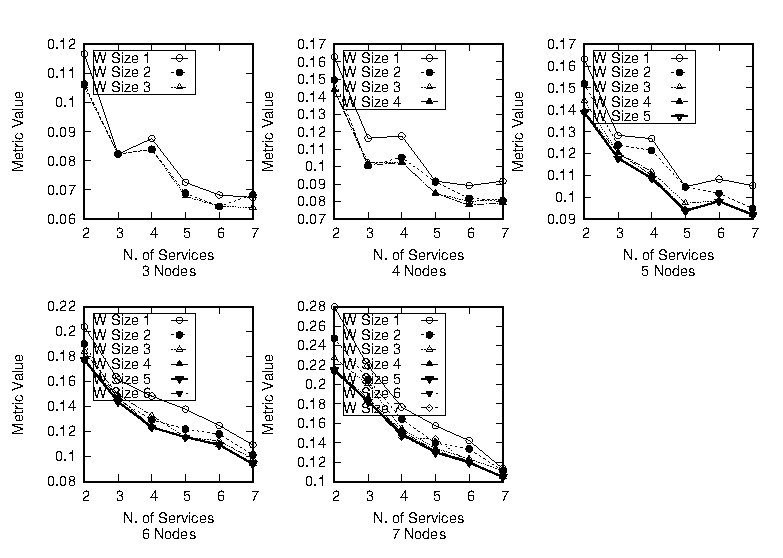
\includegraphics[height=0.3\textheight]{graphs/window_quality.eps}

    \caption{Services operating on the 0.2 to 0.8 data pruning range.}
    \label{fig:windows_quality_good}
  \end{subfigure}
  \hfill % adds horizontal space between the figures

  % Second figure
  \begin{subfigure}[b]{\textwidth}
    \centering
    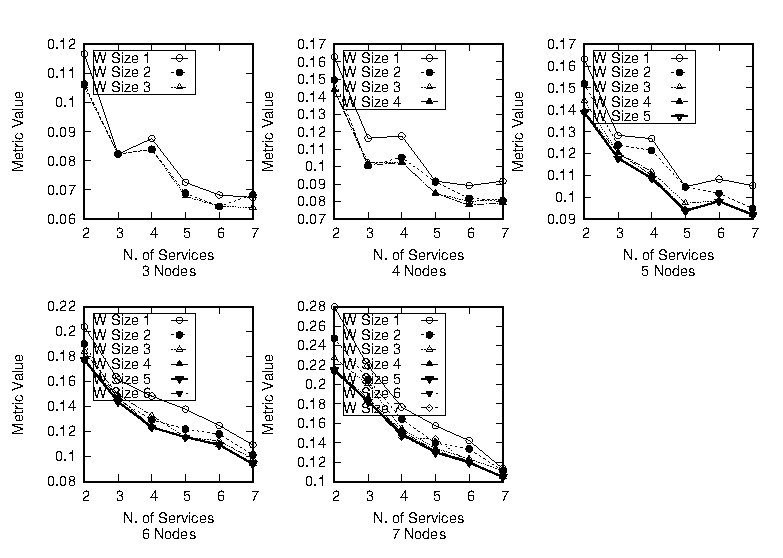
\includegraphics[height=0.3\textheight]{graphs/window_quality.eps}

    \caption{Services operating on the 0.2 to 0.5 data pruning range.}
    \label{fig:second}
  \end{subfigure}
  \hfill % adds horizontal space between the figures

  % Third figure
  \begin{subfigure}[b]{\textwidth}
    \centering
    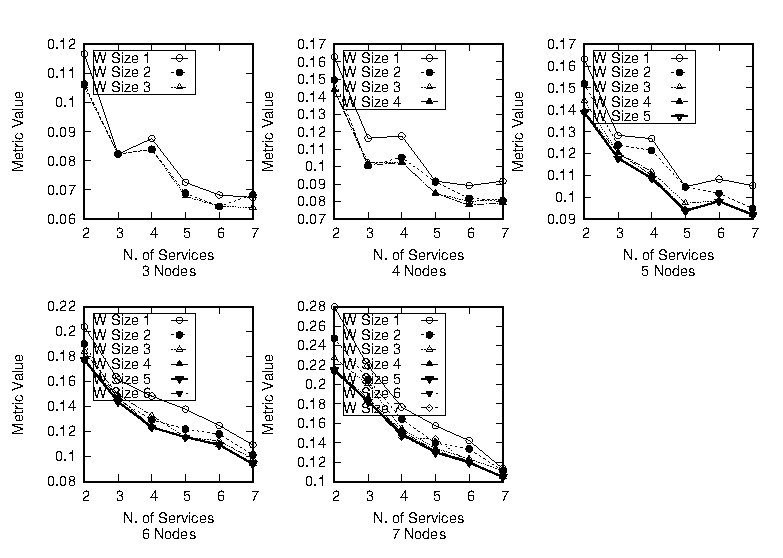
\includegraphics[height=0.3\textheight]{graphs/window_quality.eps}

    \caption{Services operating on the 0.2 to 1 data pruning range.}
    \label{fig:third}
  \end{subfigure}

  \caption{Three figures side by side}
  \label{fig:quality_window}

\end{figure*}

\section{Related Work}\label{sec:related}

% \begin{itemize}
% \item We believe that the closest approach to the one in this paper is the work of Hu et al. \cite{HUFerraiolo:2014}, introducing a generalised access control model for big data processing frameworks, which can be extended to the Hadoop environment. However, the paper discusses the issues only from a high-level architectural point of view, without discussing a tangible solution.
% \item \cite{GuardSpark:ACSAC:2020}  purpose-aware access control model, where purposes are data processing purpose and data operation purpose; the enforcement mechanism, still based on yes/no answer is based on an algorithm that checks if the operation on data to be performed matches to the purpose. The examples are given only for structured data and SQL queries. E se da una parte fa piu' di altri, dall'altra non ci sono attributi associati ai soggetti e agli oggetti, cosa che limita un pochino.
% \item \cite{Sandhu:ABAC:2018} propose a solution specifically tailored to the Apache Hadoop stack, una semplice formalizzazione dell'AC in Hadoop. Non considerano la messa in sicurezza dell'ingestion time e non considerano la questione delle coalizioni. Considerano solo servizi all'interno di Hadoop ecosystem. Classica risposta yes/no.
% \item \cite{ABACforHBase:2019} questo e' solo su HBase
% \end{itemize}

\section{Conclusions}
\clearpage
%\bibliographystyle{spbasic}      % basic style, author-year citations
\bibliographystyle{spmpsci}      % mathematics and physical sciences
%\bibliographystyle{spphys}       % APS-like style for physics
\bibliography{bib_on_BigDataAccessControl}   % name your BibTeX data base

\end{document}


